\section{Construção de árvores sintáticas}

\begin{frame}[fragile]{Construção de árvores sintáticas para expressões}

    \begin{itemize}
        \item Árvores sintáticas para expressões podem ser construídas de forma semelhante à tradução para notação posfixa
        \pause

        \item Deve ser construído um nó para cada operação e cada operando
        \pause

        \item Os filhos do nó de um operador ser subárvores que representam as subexpressões que constituem os operandos daquele operador
        \pause

        \item Cada nó pode ser implementado como um registro com vários campos que caracterizam o nó
        \pause

        \item O registro de nós que representam operadores devem conter um campo que identifica o operador e os demais campos devem ser ponteiros para os
            operandos
        \pause

        \item As folhas das árvores contém os tokens
        \pause

        \item O registro de uma folha deve identificar o token e também armazenar um ponteiro para a entrada do token na tabela de símbolos
    \end{itemize}

\end{frame}

\begin{frame}[fragile]{Funções para a criação de nós da árvore sintática de uma expressão}

    Cada uma das funções abaixo retorna um ponteiro para o nó criado. Assuma que os operadores são todos binários.
    \vspace{0.2in}
    \pause

    \begin{enumerate}
        \item \Call{criarNo}{$op, L, R$}: cria um nó de operador cujo rótulo é $op$, $L$ é o ponteiro do operando à esquerda e $R$ o ponteiro do operando à
            direita
        \pause

        \item \Call{criarFolha}{\textbf{id}, $p$}: cria um nó para um identificador com rótulo \textbf{id}, onde $p$ é o ponteiro para o identificador na tabela 
            de símbolos
        \pause

        \item \Call{criarFolha}{\textbf{num}, $val$}: cria um nó para um número, com rótulo \textbf{num}, cujo valor é indicado por $val$
    \end{enumerate}

\end{frame}

\begin{frame}[fragile]{Criação da árvore sintática da expressão \code{apl}{a - 4 + c}}

    \begin{tikzpicture}
        \node[opacity=0] at (0, 0) { y };
        \node[opacity=0] at (14, 7) { t };

        \node[anchor=west] at (0, 6) { \textbf{Chamadas de funções} };
    \end{tikzpicture}

\end{frame}

\begin{frame}[fragile]{Criação da árvore sintática da expressão \code{apl}{a - 4 + c}}

    \begin{tikzpicture}
        \node[opacity=0] at (0, 0) { y };
        \node[opacity=0] at (14, 7) { t };

        \node[anchor=west] at (0, 6) { \textbf{Chamadas de funções} };
        \node[anchor=west] at (0.5, 5) { $p_1 := \Call{criarFolha}{\textbf{id}, p_a}$ };
    \end{tikzpicture}

\end{frame}

\begin{frame}[fragile]{Criação da árvore sintática da expressão \code{apl}{a - 4 + c}}

    \begin{tikzpicture}
        \node[opacity=0] at (0, 0) { y };
        \node[opacity=0] at (14, 7) { t };

        \node[anchor=west] at (0, 6) { \textbf{Chamadas de funções} };
        \node[anchor=west] at (0.5, 5) { $p_1 := \Call{criarFolha}{\textbf{id}, p_a}$ };

        \draw[thick] (6, 2) rectangle (6.75, 2.75);
        \node at (6.375, 2.375) { \footnotesize \textbf{id} };
        \draw[thick] (6.75, 2) rectangle (7.5, 2.75);
        \draw[thick,-latex] (7.125, 2.375) to (7.125, 1.5);
        \node at (7.125, 1.35) { \footnotesize $p_a$ };

    \end{tikzpicture}

\end{frame}

\begin{frame}[fragile]{Criação da árvore sintática da expressão \code{apl}{a - 4 + c}}

    \begin{tikzpicture}
        \node[opacity=0] at (0, 0) { y };
        \node[opacity=0] at (14, 7) { t };

        \node[anchor=west] at (0, 6) { \textbf{Chamadas de funções} };
        \node[anchor=west] at (0.5, 5) { $p_1 := \Call{criarFolha}{\textbf{id}, p_a}$ };
        \node[anchor=west] at (0.5, 4.5) { $p_2 := \Call{criarFolha}{\textbf{num}, 4}$ };

        \draw[thick] (6, 2) rectangle (6.75, 2.75);
        \node at (6.375, 2.375) { \footnotesize \textbf{id} };
        \draw[thick] (6.75, 2) rectangle (7.5, 2.75);
        \draw[thick,-latex] (7.125, 2.375) to (7.125, 1.5);
        \node at (7.125, 1.35) { \footnotesize $p_a$ };

    \end{tikzpicture}

\end{frame}

\begin{frame}[fragile]{Criação da árvore sintática da expressão \code{apl}{a - 4 + c}}

    \begin{tikzpicture}
        \node[opacity=0] at (0, 0) { y };
        \node[opacity=0] at (14, 7) { t };

        \node[anchor=west] at (0, 6) { \textbf{Chamadas de funções} };
        \node[anchor=west] at (0.5, 5) { $p_1 := \Call{criarFolha}{\textbf{id}, p_a}$ };
        \node[anchor=west] at (0.5, 4.5) { $p_2 := \Call{criarFolha}{\textbf{num}, 4}$ };

        \draw[thick] (6, 2) rectangle (6.75, 2.75);
        \node at (6.375, 2.375) { \footnotesize \textbf{id} };
        \draw[thick] (6.75, 2) rectangle (7.5, 2.75);
        \draw[thick,-latex] (7.125, 2.375) to (7.125, 1.5);
        \node at (7.125, 1.35) { \footnotesize $p_a$ };
        \draw[thick] (9.75, 2) rectangle (10.5, 2.75);
        \node at (10.125, 2.375) { \footnotesize \textbf{num} };
        \draw[thick] (10.5, 2) rectangle (11.25, 2.75);
        \node at (10.875, 2.375) { \footnotesize $4$ };
%        \draw[thick] (7.5, 4) rectangle (8.25, 4.75);
%        \draw[thick] (8.25, 4) rectangle (9, 4.75);
%        \draw[thick] (9, 4) rectangle (9.75, 4.75);
%        \draw[thick] (9.75, 6) rectangle (10.5, 6.75);
%        \draw[thick] (10.5, 6) rectangle (11.25, 6.75);
%        \draw[thick] (11.25, 6) rectangle (12, 6.75);
%        \draw[thick] (12, 4) rectangle (12.75, 4.75);
%        \draw[thick] (12.75, 4) rectangle (13.5, 4.75);

    \end{tikzpicture}

\end{frame}

\begin{frame}[fragile]{Criação da árvore sintática da expressão \code{apl}{a - 4 + c}}

    \begin{tikzpicture}
        \node[opacity=0] at (0, 0) { y };
        \node[opacity=0] at (14, 7) { t };

        \node[anchor=west] at (0, 6) { \textbf{Chamadas de funções} };
        \node[anchor=west] at (0.5, 5) { $p_1 := \Call{criarFolha}{\textbf{id}, p_a}$ };
        \node[anchor=west] at (0.5, 4.5) { $p_2 := \Call{criarFolha}{\textbf{num}, 4}$ };
        \node[anchor=west] at (0.5, 4) { $p_3 := \Call{criarNo}{\code{apl}{+}, p_1, p_2}$ };

        \draw[thick] (6, 2) rectangle (6.75, 2.75);
        \node at (6.375, 2.375) { \footnotesize \textbf{id} };
        \draw[thick] (6.75, 2) rectangle (7.5, 2.75);
        \draw[thick,-latex] (7.125, 2.375) to (7.125, 1.5);
        \node at (7.125, 1.35) { \footnotesize $p_a$ };
        \draw[thick] (9.75, 2) rectangle (10.5, 2.75);
        \node at (10.125, 2.375) { \footnotesize \textbf{num} };
        \draw[thick] (10.5, 2) rectangle (11.25, 2.75);
        \node at (10.875, 2.375) { \footnotesize $4$ };
%        \draw[thick] (7.5, 4) rectangle (8.25, 4.75);
%        \draw[thick] (8.25, 4) rectangle (9, 4.75);
%        \draw[thick] (9, 4) rectangle (9.75, 4.75);
%        \draw[thick] (9.75, 6) rectangle (10.5, 6.75);
%        \draw[thick] (10.5, 6) rectangle (11.25, 6.75);
%        \draw[thick] (11.25, 6) rectangle (12, 6.75);
%        \draw[thick] (12, 4) rectangle (12.75, 4.75);
%        \draw[thick] (12.75, 4) rectangle (13.5, 4.75);

    \end{tikzpicture}

\end{frame}

\begin{frame}[fragile]{Criação da árvore sintática da expressão \code{apl}{a - 4 + c}}

    \begin{tikzpicture}
        \node[opacity=0] at (0, 0) { y };
        \node[opacity=0] at (14, 7) { t };

        \node[anchor=west] at (0, 6) { \textbf{Chamadas de funções} };
        \node[anchor=west] at (0.5, 5) { $p_1 := \Call{criarFolha}{\textbf{id}, p_a}$ };
        \node[anchor=west] at (0.5, 4.5) { $p_2 := \Call{criarFolha}{\textbf{num}, 4}$ };
        \node[anchor=west] at (0.5, 4) { $p_3 := \Call{criarNo}{\code{apl}{+}, p_1, p_2}$ };

        \draw[thick] (6, 2) rectangle (6.75, 2.75);
        \node at (6.375, 2.375) { \footnotesize \textbf{id} };
        \draw[thick] (6.75, 2) rectangle (7.5, 2.75);
        \draw[thick,-latex] (7.125, 2.375) to (7.125, 1.5);
        \node at (7.125, 1.35) { \footnotesize $p_a$ };
        \draw[thick] (9.75, 2) rectangle (10.5, 2.75);
        \node at (10.125, 2.375) { \footnotesize \textbf{num} };
        \draw[thick] (10.5, 2) rectangle (11.25, 2.75);
        \node at (10.875, 2.375) { \footnotesize $4$ };
        \draw[thick] (7.5, 4) rectangle (8.25, 4.75);
        \node at (7.875, 4.375) { \code{apl}{+} };
        \draw[thick] (8.25, 4) rectangle (9, 4.75);
        \draw[-latex, thick] (8.675, 4.375) .. controls (8.675, 3.25) and (6.75, 3.5) .. (6.75, 2.75);
        \draw[thick] (9, 4) rectangle (9.75, 4.75);
        \draw[-latex, thick] (9.375, 4.375) .. controls (9.375, 3.25) and (10.5, 3.5) .. (10.5, 2.75);
%        \draw[thick] (9.75, 6) rectangle (10.5, 6.75);
%        \draw[thick] (10.5, 6) rectangle (11.25, 6.75);
%        \draw[thick] (11.25, 6) rectangle (12, 6.75);
%        \draw[thick] (12, 4) rectangle (12.75, 4.75);
%        \draw[thick] (12.75, 4) rectangle (13.5, 4.75);

    \end{tikzpicture}

\end{frame}

\begin{frame}[fragile]{Criação da árvore sintática da expressão \code{apl}{a - 4 + c}}

    \begin{tikzpicture}
        \node[opacity=0] at (0, 0) { y };
        \node[opacity=0] at (14, 7) { t };

        \node[anchor=west] at (0, 6) { \textbf{Chamadas de funções} };
        \node[anchor=west] at (0.5, 5) { $p_1 := \Call{criarFolha}{\textbf{id}, p_a}$ };
        \node[anchor=west] at (0.5, 4.5) { $p_2 := \Call{criarFolha}{\textbf{num}, 4}$ };
        \node[anchor=west] at (0.5, 4) { $p_3 := \Call{criarNo}{\code{apl}{+}, p_1, p_2}$ };
        \node[anchor=west] at (0.5, 3.5) { $p_4 := \Call{criarFolha}{\textbf{id}, p_c}$ };

        \draw[thick] (6, 2) rectangle (6.75, 2.75);
        \node at (6.375, 2.375) { \footnotesize \textbf{id} };
        \draw[thick] (6.75, 2) rectangle (7.5, 2.75);
        \draw[thick,-latex] (7.125, 2.375) to (7.125, 1.5);
        \node at (7.125, 1.35) { \footnotesize $p_a$ };
        \draw[thick] (9.75, 2) rectangle (10.5, 2.75);
        \node at (10.125, 2.375) { \footnotesize \textbf{num} };
        \draw[thick] (10.5, 2) rectangle (11.25, 2.75);
        \node at (10.875, 2.375) { \footnotesize $4$ };
        \draw[thick] (7.5, 4) rectangle (8.25, 4.75);
        \node at (7.875, 4.375) { \code{apl}{+} };
        \draw[thick] (8.25, 4) rectangle (9, 4.75);
        \draw[-latex, thick] (8.675, 4.375) .. controls (8.675, 3.25) and (6.75, 3.5) .. (6.75, 2.75);
        \draw[thick] (9, 4) rectangle (9.75, 4.75);
        \draw[-latex, thick] (9.375, 4.375) .. controls (9.375, 3.25) and (10.5, 3.5) .. (10.5, 2.75);
%        \draw[thick] (9.75, 6) rectangle (10.5, 6.75);
%        \draw[thick] (10.5, 6) rectangle (11.25, 6.75);
%        \draw[thick] (11.25, 6) rectangle (12, 6.75);
%        \draw[thick] (12, 4) rectangle (12.75, 4.75);
%        \draw[thick] (12.75, 4) rectangle (13.5, 4.75);

    \end{tikzpicture}

\end{frame}

\begin{frame}[fragile]{Criação da árvore sintática da expressão \code{apl}{a - 4 + c}}

    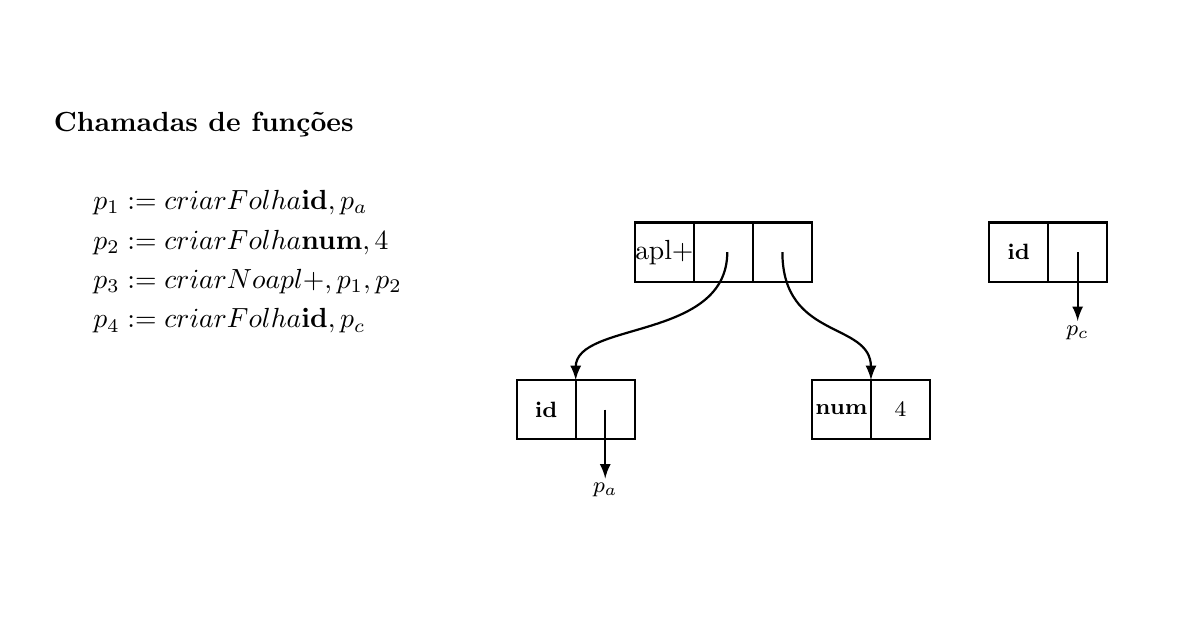
\begin{tikzpicture}
        \node[opacity=0] at (0, 0) { y };
        \node[opacity=0] at (14, 7) { t };

        \node[anchor=west] at (0, 6) { \textbf{Chamadas de funções} };
        \node[anchor=west] at (0.5, 5) { $p_1 := \Call{criarFolha}{\textbf{id}, p_a}$ };
        \node[anchor=west] at (0.5, 4.5) { $p_2 := \Call{criarFolha}{\textbf{num}, 4}$ };
        \node[anchor=west] at (0.5, 4) { $p_3 := \Call{criarNo}{\code{apl}{+}, p_1, p_2}$ };
        \node[anchor=west] at (0.5, 3.5) { $p_4 := \Call{criarFolha}{\textbf{id}, p_c}$ };

        \draw[thick] (6, 2) rectangle (6.75, 2.75);
        \node at (6.375, 2.375) { \footnotesize \textbf{id} };
        \draw[thick] (6.75, 2) rectangle (7.5, 2.75);
        \draw[thick,-latex] (7.125, 2.375) to (7.125, 1.5);
        \node at (7.125, 1.35) { \footnotesize $p_a$ };
        \draw[thick] (9.75, 2) rectangle (10.5, 2.75);
        \node at (10.125, 2.375) { \footnotesize \textbf{num} };
        \draw[thick] (10.5, 2) rectangle (11.25, 2.75);
        \node at (10.875, 2.375) { \footnotesize $4$ };
        \draw[thick] (7.5, 4) rectangle (8.25, 4.75);
        \node at (7.875, 4.375) { \code{apl}{+} };
        \draw[thick] (8.25, 4) rectangle (9, 4.75);
        \draw[-latex, thick] (8.675, 4.375) .. controls (8.675, 3.25) and (6.75, 3.5) .. (6.75, 2.75);
        \draw[thick] (9, 4) rectangle (9.75, 4.75);
        \draw[-latex, thick] (9.375, 4.375) .. controls (9.375, 3.25) and (10.5, 3.5) .. (10.5, 2.75);
%        \draw[thick] (9.75, 6) rectangle (10.5, 6.75);
%        \draw[thick] (10.5, 6) rectangle (11.25, 6.75);
%        \draw[thick] (11.25, 6) rectangle (12, 6.75);
        \draw[thick] (12, 4) rectangle (12.75, 4.75);
        \node at (12.375, 4.375) { \footnotesize \textbf{id} };
        \draw[thick] (12.75, 4) rectangle (13.5, 4.75);
        \draw[thick,-latex] (13.125, 4.375) to (13.125, 3.5);
        \node at (13.125, 3.35) { \footnotesize $p_c$ };

    \end{tikzpicture}

\end{frame}

\begin{frame}[fragile]{Criação da árvore sintática da expressão \code{apl}{a - 4 + c}}

    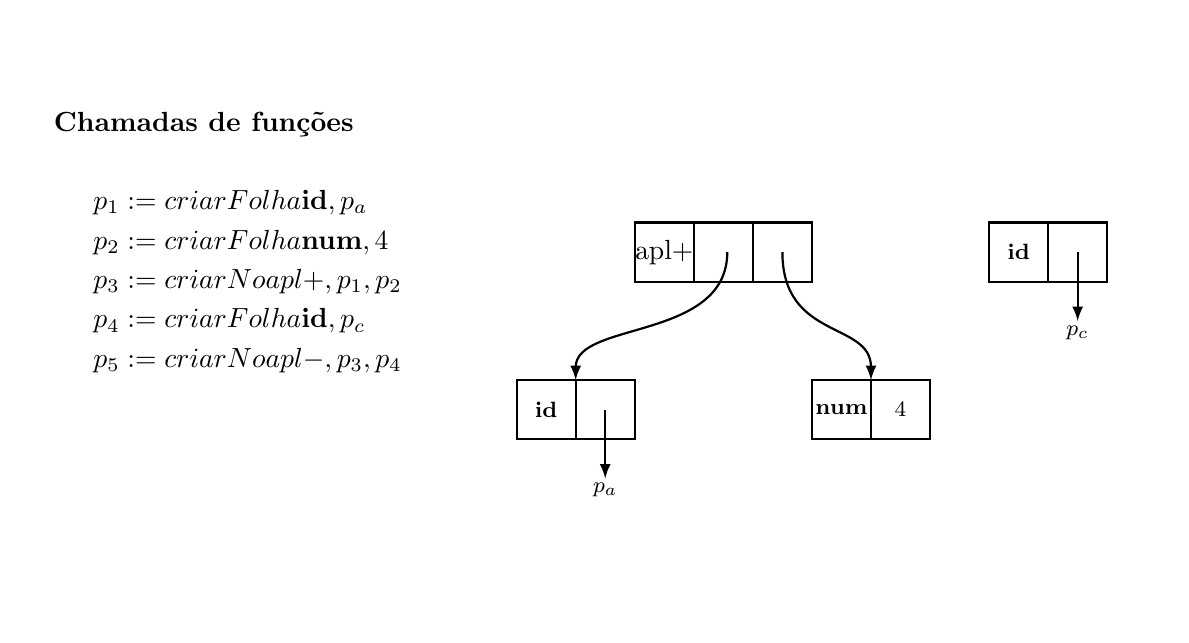
\begin{tikzpicture}
        \node[opacity=0] at (0, 0) { y };
        \node[opacity=0] at (14, 7) { t };

        \node[anchor=west] at (0, 6) { \textbf{Chamadas de funções} };
        \node[anchor=west] at (0.5, 5) { $p_1 := \Call{criarFolha}{\textbf{id}, p_a}$ };
        \node[anchor=west] at (0.5, 4.5) { $p_2 := \Call{criarFolha}{\textbf{num}, 4}$ };
        \node[anchor=west] at (0.5, 4) { $p_3 := \Call{criarNo}{\code{apl}{+}, p_1, p_2}$ };
        \node[anchor=west] at (0.5, 3.5) { $p_4 := \Call{criarFolha}{\textbf{id}, p_c}$ };
        \node[anchor=west] at (0.5, 3) { $p_5 := \Call{criarNo}{\code{apl}{-}, p_3, p_4}$ };

        \draw[thick] (6, 2) rectangle (6.75, 2.75);
        \node at (6.375, 2.375) { \footnotesize \textbf{id} };
        \draw[thick] (6.75, 2) rectangle (7.5, 2.75);
        \draw[thick,-latex] (7.125, 2.375) to (7.125, 1.5);
        \node at (7.125, 1.35) { \footnotesize $p_a$ };
        \draw[thick] (9.75, 2) rectangle (10.5, 2.75);
        \node at (10.125, 2.375) { \footnotesize \textbf{num} };
        \draw[thick] (10.5, 2) rectangle (11.25, 2.75);
        \node at (10.875, 2.375) { \footnotesize $4$ };
        \draw[thick] (7.5, 4) rectangle (8.25, 4.75);
        \node at (7.875, 4.375) { \code{apl}{+} };
        \draw[thick] (8.25, 4) rectangle (9, 4.75);
        \draw[-latex, thick] (8.675, 4.375) .. controls (8.675, 3.25) and (6.75, 3.5) .. (6.75, 2.75);
        \draw[thick] (9, 4) rectangle (9.75, 4.75);
        \draw[-latex, thick] (9.375, 4.375) .. controls (9.375, 3.25) and (10.5, 3.5) .. (10.5, 2.75);
%        \draw[thick] (9.75, 6) rectangle (10.5, 6.75);
%        \draw[thick] (10.5, 6) rectangle (11.25, 6.75);
%        \draw[thick] (11.25, 6) rectangle (12, 6.75);
        \draw[thick] (12, 4) rectangle (12.75, 4.75);
        \node at (12.375, 4.375) { \footnotesize \textbf{id} };
        \draw[thick] (12.75, 4) rectangle (13.5, 4.75);
        \draw[thick,-latex] (13.125, 4.375) to (13.125, 3.5);
        \node at (13.125, 3.35) { \footnotesize $p_c$ };

    \end{tikzpicture}

\end{frame}

\begin{frame}[fragile]{Criação da árvore sintática da expressão \code{apl}{a - 4 + c}}

    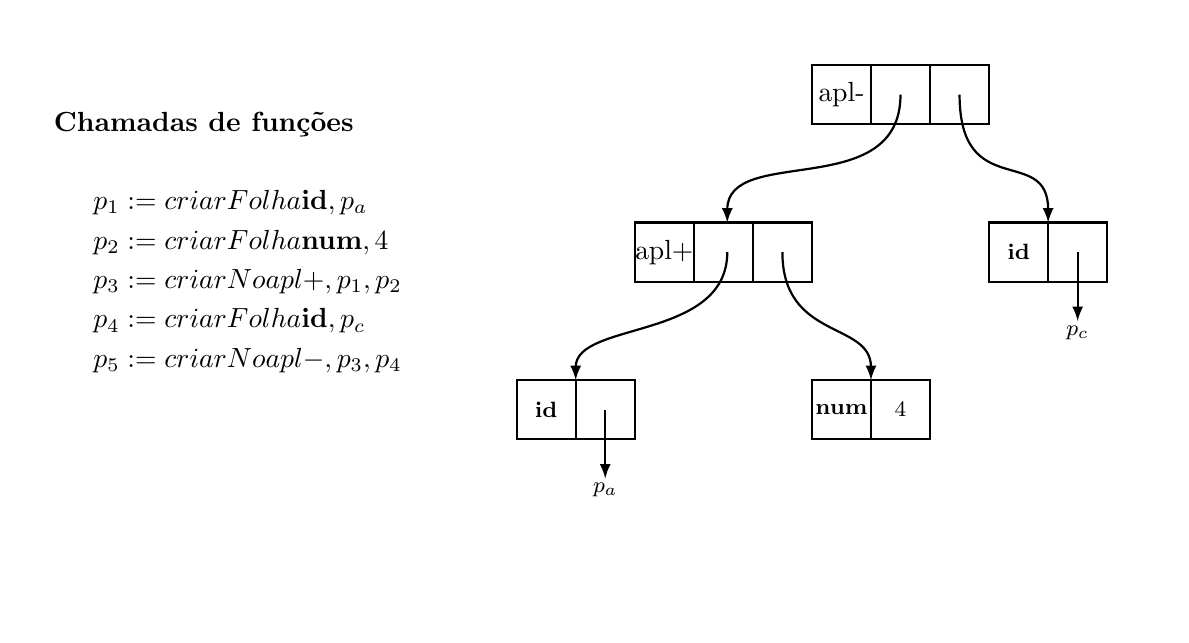
\begin{tikzpicture}
        \node[opacity=0] at (0, 0) { y };
        \node[opacity=0] at (14, 7) { t };

        \node[anchor=west] at (0, 6) { \textbf{Chamadas de funções} };
        \node[anchor=west] at (0.5, 5) { $p_1 := \Call{criarFolha}{\textbf{id}, p_a}$ };
        \node[anchor=west] at (0.5, 4.5) { $p_2 := \Call{criarFolha}{\textbf{num}, 4}$ };
        \node[anchor=west] at (0.5, 4) { $p_3 := \Call{criarNo}{\code{apl}{+}, p_1, p_2}$ };
        \node[anchor=west] at (0.5, 3.5) { $p_4 := \Call{criarFolha}{\textbf{id}, p_c}$ };
        \node[anchor=west] at (0.5, 3) { $p_5 := \Call{criarNo}{\code{apl}{-}, p_3, p_4}$ };

        \draw[thick] (6, 2) rectangle (6.75, 2.75);
        \node at (6.375, 2.375) { \footnotesize \textbf{id} };
        \draw[thick] (6.75, 2) rectangle (7.5, 2.75);
        \draw[thick,-latex] (7.125, 2.375) to (7.125, 1.5);
        \node at (7.125, 1.35) { \footnotesize $p_a$ };
        \draw[thick] (9.75, 2) rectangle (10.5, 2.75);
        \node at (10.125, 2.375) { \footnotesize \textbf{num} };
        \draw[thick] (10.5, 2) rectangle (11.25, 2.75);
        \node at (10.875, 2.375) { \footnotesize $4$ };
        \draw[thick] (7.5, 4) rectangle (8.25, 4.75);
        \node at (7.875, 4.375) { \code{apl}{+} };
        \draw[thick] (8.25, 4) rectangle (9, 4.75);
        \draw[-latex, thick] (8.675, 4.375) .. controls (8.675, 3.25) and (6.75, 3.5) .. (6.75, 2.75);
        \draw[thick] (9, 4) rectangle (9.75, 4.75);
        \draw[-latex, thick] (9.375, 4.375) .. controls (9.375, 3.25) and (10.5, 3.5) .. (10.5, 2.75);
        \draw[thick] (9.75, 6) rectangle (10.5, 6.75);
        \node at (10.125, 6.375) { \code{apl}{-} };
        \draw[thick] (10.5, 6) rectangle (11.25, 6.75);
        \draw[-latex, thick] (10.875, 6.375) .. controls (10.875, 5) and (8.675, 5.75) .. (8.675, 4.75);
        \draw[thick] (11.25, 6) rectangle (12, 6.75);
        \draw[-latex, thick] (11.625, 6.375) .. controls (11.625, 5) and (12.75, 5.75) .. (12.75, 4.75);
        \draw[thick] (12, 4) rectangle (12.75, 4.75);
        \node at (12.375, 4.375) { \footnotesize \textbf{id} };
        \draw[thick] (12.75, 4) rectangle (13.5, 4.75);
        \draw[thick,-latex] (13.125, 4.375) to (13.125, 3.5);
        \node at (13.125, 3.35) { \footnotesize $p_c$ };

    \end{tikzpicture}

\end{frame}


\begin{frame}[fragile]{Definição dirigida pela sintaxe para a construção de árvores sintáticas}

    \begin{itemize}
        \item É possível construir árvores sintáticas para expressões por meio de uma definição S-atribuída
        \pause

        \item As regras semânticas agendam as chamadas das funções de criação de nós que irão construir a árvore
        \pause

        \item O atributo sintetizado $nptr$ controla os ponteiros para os nós retornados pelas funções
        \pause

        \item O atributo $entrada$ armazena o endereço de um token na tabela de símbolos e o atributo $val$ o valor de um número
        \pause

        \item Estes dois atributos devem ser computados na análise léxica
    \end{itemize}

\end{frame}

\begin{frame}[fragile]{Definição dirigida pela sintaxe para expressões aritméticas de adição e subtração}

    \begin{table}
        \centering
        \begin{tabular}{lp{2cm}l}
        \toprule
        \textbf{Produção} & & \textbf{Regra semântica} \\
        \midrule
        $E\to E_1\ \code{apl}{+}\ T$ & & $E.nptr := \Call{criarNo}{\code{apl}{+}, E_1.nptr, T.nptr}$ \\
        \rowcolor[gray]{0.9}
        $E\to E_1\ \code{apl}{-}\ T$ & & $E.nptr := \Call{criarNo}{\code{apl}{-}, E_1.nptr, T.nptr}$ \\
        $E\to T$ & & $E.nptr := T.nptr$ \\
        \rowcolor[gray]{0.9}
        $T\to (E)$ & & $T.nptr := E.nptr$ \\
        $T\to \textbf{id}$ & & $T.nptr := \Call{criarNo}{\textbf{id}, \textbf{id}.entrada}$ \\
        \rowcolor[gray]{0.9}
        $T\to \textbf{num}$ & & $T.nptr := \Call{criarNo}{\textbf{num}, \textbf{num}.val}$ \\
        \bottomrule
        \end{tabular} 
    \end{table}

\end{frame}

\begin{frame}[fragile]{DAG}

    \begin{itemize}
        \item Um grafo direcionado acíclico (\textit{directed acyclic graph -- DAG}) é um grafo cujas arestas são direcionadas e que não possui ciclos
        \pause

        \item Um DAG pode ser usado para identificar subexpressões comuns em uma expressão
        \pause

        \item De forma similar às árvores sintáticas, um nó representa um operador e seus filhos representam os operandos
        \pause

        \item Se houver uma ou mais expressões comuns, os nós do DAG podem ter ``mais de um pai''
        \pause

        \item Nas árvores sintáticas, expressões comuns são duplicadas na árvore
    \end{itemize}

\end{frame}

\begin{frame}[fragile]{Construção do DAG a partir de uma definição S-atribuída}

    \begin{itemize}
        \item Uma definição S-atribuída para a construção de árvores sintáticas para expressões aritméticas de adições e subtrações pode se adaptada para a 
            construção do DAG
        \pause

        \item De fato, basta modificar o comportamento das funções \Call{criarNo}{\ } e \Call{criarFolha}{\ }
        \pause

        \item Ao invés de criar um novo nó a cada chamada, estas funções devem verificar se os parâmatros passados já não foram usados para construir um nó
        \pause

        \item Em caso afirmativo, as funções devem retornar o ponteiro usado anteriormente na criação do nó
        \pause

        \item Caso contrário, deve ser criado um novo nó e o ponteiro criado deve ser armazenado em uma tabela, associado aos parâmetros usados, para consulta
            posterior
    \end{itemize}

\end{frame}

\begin{frame}[fragile]{Criação do DAG para a expressão \code{apl}{a + a × (b - c) + (b - c) × d}}

    \begin{tikzpicture}
        \node[opacity=0] at (0, 0) { y };
        \node[opacity=0] at (14, 7) { t };

        \node[anchor=west] at (0, 6.75) { \textbf{Chamadas de funções} };
    \end{tikzpicture}

\end{frame}

\begin{frame}[fragile]{Criação do DAG para a expressão \code{apl}{a + a × (b - c) + (b - c) × d}}

    \begin{tikzpicture}
        \node[opacity=0] at (0, 0) { y };
        \node[opacity=0] at (14, 7) { t };

        \node[anchor=west] at (0, 6.75) { \textbf{Chamadas de funções} };
        \node[anchor=west] at (0.5, 6.0) { $p_1 := \Call{criarFolha}{\textbf{id}, p_a}$ };
%        \node[anchor=west] at (0.5, 5.5) { $p_2 := \Call{criarFolha}{\textbf{id}, p_a}$ };
%        \node[anchor=west] at (0.5, 5.0) { $p_3 := \Call{criarFolha}{\textbf{id}, p_a}$ };
%        \node[anchor=west] at (0.5, 4.5) { $p_4 := \Call{criarFolha}{\textbf{id}, p_a}$ };
%        \node[anchor=west] at (0.5, 4.0) { $p_5 := \Call{criarFolha}{\textbf{id}, p_a}$ };
%        \node[anchor=west] at (0.5, 3.5) { $p_6 := \Call{criarFolha}{\textbf{id}, p_a}$ };
%        \node[anchor=west] at (0.5, 3.0) { $p_7 := \Call{criarFolha}{\textbf{id}, p_a}$ };
%        \node[anchor=west] at (0.5, 2.5) { $p_8 := \Call{criarFolha}{\textbf{id}, p_a}$ };
%        \node[anchor=west] at (0.5, 2.0) { $p_9 := \Call{criarFolha}{\textbf{id}, p_a}$ };
%        \node[anchor=west] at (0.5, 1.5) { $p_10 := \Call{criarFolha}{\textbf{id}, p_a}$ };
%        \node[anchor=west] at (0.5, 1.0) { $p_11 := \Call{criarFolha}{\textbf{id}, p_a}$ };
%        \node[anchor=west] at (0.5, 0.5) { $p_12 := \Call{criarFolha}{\textbf{id}, p_a}$ };
%        \node[anchor=west] at (0.5, 0.0) { $p_13 := \Call{criarFolha}{\textbf{id}, p_a}$ };

    \end{tikzpicture}

\end{frame}

\begin{frame}[fragile]{Criação do DAG para a expressão \code{apl}{a + a × (b - c) + (b - c) × d}}

    \begin{tikzpicture}
        \node[opacity=0] at (0, 0) { y };
        \node[opacity=0] at (14, 7) { t };

        \node[anchor=west] at (0, 6.75) { \textbf{Chamadas de funções} };
        \node[anchor=west] at (0.5, 6.0) { $p_1 := \Call{criarFolha}{\textbf{id}, p_a}$ };
%        \node[anchor=west] at (0.5, 5.5) { $p_2 := \Call{criarFolha}{\textbf{id}, p_a}$ };
%        \node[anchor=west] at (0.5, 5.0) { $p_3 := \Call{criarFolha}{\textbf{id}, p_a}$ };
%        \node[anchor=west] at (0.5, 4.5) { $p_4 := \Call{criarFolha}{\textbf{id}, p_a}$ };
%        \node[anchor=west] at (0.5, 4.0) { $p_5 := \Call{criarFolha}{\textbf{id}, p_a}$ };
%        \node[anchor=west] at (0.5, 3.5) { $p_6 := \Call{criarFolha}{\textbf{id}, p_a}$ };
%        \node[anchor=west] at (0.5, 3.0) { $p_7 := \Call{criarFolha}{\textbf{id}, p_a}$ };
%        \node[anchor=west] at (0.5, 2.5) { $p_8 := \Call{criarFolha}{\textbf{id}, p_a}$ };
%        \node[anchor=west] at (0.5, 2.0) { $p_9 := \Call{criarFolha}{\textbf{id}, p_a}$ };
%        \node[anchor=west] at (0.5, 1.5) { $p_10 := \Call{criarFolha}{\textbf{id}, p_a}$ };
%        \node[anchor=west] at (0.5, 1.0) { $p_11 := \Call{criarFolha}{\textbf{id}, p_a}$ };
%        \node[anchor=west] at (0.5, 0.5) { $p_12 := \Call{criarFolha}{\textbf{id}, p_a}$ };
%        \node[anchor=west] at (0.5, 0.0) { $p_13 := \Call{criarFolha}{\textbf{id}, p_a}$ };

        \node (A) at (8, 2) { \Large \code{apl}{a} };

    \end{tikzpicture}

\end{frame}

\begin{frame}[fragile]{Criação do DAG para a expressão \code{apl}{a + a × (b - c) + (b - c) × d}}

    \begin{tikzpicture}
        \node[opacity=0] at (0, 0) { y };
        \node[opacity=0] at (14, 7) { t };

        \node[anchor=west] at (0, 6.75) { \textbf{Chamadas de funções} };
        \node[anchor=west] at (0.5, 6.0) { $p_1 := \Call{criarFolha}{\textbf{id}, p_a}$ };
        \node[anchor=west] at (0.5, 5.5) { $p_2 := \Call{criarFolha}{\textbf{id}, p_a}$ };
%        \node[anchor=west] at (0.5, 5.0) { $p_3 := \Call{criarFolha}{\textbf{id}, p_a}$ };
%        \node[anchor=west] at (0.5, 4.5) { $p_4 := \Call{criarFolha}{\textbf{id}, p_a}$ };
%        \node[anchor=west] at (0.5, 4.0) { $p_5 := \Call{criarFolha}{\textbf{id}, p_a}$ };
%        \node[anchor=west] at (0.5, 3.5) { $p_6 := \Call{criarFolha}{\textbf{id}, p_a}$ };
%        \node[anchor=west] at (0.5, 3.0) { $p_7 := \Call{criarFolha}{\textbf{id}, p_a}$ };
%        \node[anchor=west] at (0.5, 2.5) { $p_8 := \Call{criarFolha}{\textbf{id}, p_a}$ };
%        \node[anchor=west] at (0.5, 2.0) { $p_9 := \Call{criarFolha}{\textbf{id}, p_a}$ };
%        \node[anchor=west] at (0.5, 1.5) { $p_10 := \Call{criarFolha}{\textbf{id}, p_a}$ };
%        \node[anchor=west] at (0.5, 1.0) { $p_11 := \Call{criarFolha}{\textbf{id}, p_a}$ };
%        \node[anchor=west] at (0.5, 0.5) { $p_12 := \Call{criarFolha}{\textbf{id}, p_a}$ };
%        \node[anchor=west] at (0.5, 0.0) { $p_13 := \Call{criarFolha}{\textbf{id}, p_a}$ };

        \node (A) at (8, 2) { \Large \code{apl}{a} };

    \end{tikzpicture}

\end{frame}

\begin{frame}[fragile]{Criação do DAG para a expressão \code{apl}{a + a × (b - c) + (b - c) × d}}

    \begin{tikzpicture}
        \node[opacity=0] at (0, 0) { y };
        \node[opacity=0] at (14, 7) { t };

        \node[anchor=west] at (0, 6.75) { \textbf{Chamadas de funções} };
        \node[anchor=west] at (0.5, 6.0) { $p_1 := \Call{criarFolha}{\textbf{id}, p_a}$ };
        \node[anchor=west] at (0.5, 5.5) { $p_2 := \Call{criarFolha}{\textbf{id}, p_a}$ };
        \node[anchor=west] at (0.5, 5.0) { $p_3 := \Call{criarFolha}{\textbf{id}, p_b}$ };
%        \node[anchor=west] at (0.5, 4.5) { $p_4 := \Call{criarFolha}{\textbf{id}, p_a}$ };
%        \node[anchor=west] at (0.5, 4.0) { $p_5 := \Call{criarFolha}{\textbf{id}, p_a}$ };
%        \node[anchor=west] at (0.5, 3.5) { $p_6 := \Call{criarFolha}{\textbf{id}, p_a}$ };
%        \node[anchor=west] at (0.5, 3.0) { $p_7 := \Call{criarFolha}{\textbf{id}, p_a}$ };
%        \node[anchor=west] at (0.5, 2.5) { $p_8 := \Call{criarFolha}{\textbf{id}, p_a}$ };
%        \node[anchor=west] at (0.5, 2.0) { $p_9 := \Call{criarFolha}{\textbf{id}, p_a}$ };
%        \node[anchor=west] at (0.5, 1.5) { $p_10 := \Call{criarFolha}{\textbf{id}, p_a}$ };
%        \node[anchor=west] at (0.5, 1.0) { $p_11 := \Call{criarFolha}{\textbf{id}, p_a}$ };
%        \node[anchor=west] at (0.5, 0.5) { $p_12 := \Call{criarFolha}{\textbf{id}, p_a}$ };
%        \node[anchor=west] at (0.5, 0.0) { $p_13 := \Call{criarFolha}{\textbf{id}, p_a}$ };

        \node (A) at (8, 2) { \Large \code{apl}{a} };

    \end{tikzpicture}

\end{frame}

\begin{frame}[fragile]{Criação do DAG para a expressão \code{apl}{a + a × (b - c) + (b - c) × d}}

    \begin{tikzpicture}
        \node[opacity=0] at (0, 0) { y };
        \node[opacity=0] at (14, 7) { t };

        \node[anchor=west] at (0, 6.75) { \textbf{Chamadas de funções} };
        \node[anchor=west] at (0.5, 6.0) { $p_1 := \Call{criarFolha}{\textbf{id}, p_a}$ };
        \node[anchor=west] at (0.5, 5.5) { $p_2 := \Call{criarFolha}{\textbf{id}, p_a}$ };
        \node[anchor=west] at (0.5, 5.0) { $p_3 := \Call{criarFolha}{\textbf{id}, p_b}$ };
%        \node[anchor=west] at (0.5, 4.5) { $p_4 := \Call{criarFolha}{\textbf{id}, p_a}$ };
%        \node[anchor=west] at (0.5, 4.0) { $p_5 := \Call{criarFolha}{\textbf{id}, p_a}$ };
%        \node[anchor=west] at (0.5, 3.5) { $p_6 := \Call{criarFolha}{\textbf{id}, p_a}$ };
%        \node[anchor=west] at (0.5, 3.0) { $p_7 := \Call{criarFolha}{\textbf{id}, p_a}$ };
%        \node[anchor=west] at (0.5, 2.5) { $p_8 := \Call{criarFolha}{\textbf{id}, p_a}$ };
%        \node[anchor=west] at (0.5, 2.0) { $p_9 := \Call{criarFolha}{\textbf{id}, p_a}$ };
%        \node[anchor=west] at (0.5, 1.5) { $p_10 := \Call{criarFolha}{\textbf{id}, p_a}$ };
%        \node[anchor=west] at (0.5, 1.0) { $p_11 := \Call{criarFolha}{\textbf{id}, p_a}$ };
%        \node[anchor=west] at (0.5, 0.5) { $p_12 := \Call{criarFolha}{\textbf{id}, p_a}$ };
%        \node[anchor=west] at (0.5, 0.0) { $p_13 := \Call{criarFolha}{\textbf{id}, p_a}$ };

        \node (A) at (8, 2) { \Large \code{apl}{a} };
        \node (B) at (9, 0.5) { \Large \code{apl}{b} };

    \end{tikzpicture}

\end{frame}

\begin{frame}[fragile]{Criação do DAG para a expressão \code{apl}{a + a × (b - c) + (b - c) × d}}

    \begin{tikzpicture}
        \node[opacity=0] at (0, 0) { y };
        \node[opacity=0] at (14, 7) { t };

        \node[anchor=west] at (0, 6.75) { \textbf{Chamadas de funções} };
        \node[anchor=west] at (0.5, 6.0) { $p_1 := \Call{criarFolha}{\textbf{id}, p_a}$ };
        \node[anchor=west] at (0.5, 5.5) { $p_2 := \Call{criarFolha}{\textbf{id}, p_a}$ };
        \node[anchor=west] at (0.5, 5.0) { $p_3 := \Call{criarFolha}{\textbf{id}, p_b}$ };
        \node[anchor=west] at (0.5, 4.5) { $p_4 := \Call{criarFolha}{\textbf{id}, p_c}$ };
%        \node[anchor=west] at (0.5, 4.0) { $p_5 := \Call{criarFolha}{\textbf{id}, p_a}$ };
%        \node[anchor=west] at (0.5, 3.5) { $p_6 := \Call{criarFolha}{\textbf{id}, p_a}$ };
%        \node[anchor=west] at (0.5, 3.0) { $p_7 := \Call{criarFolha}{\textbf{id}, p_a}$ };
%        \node[anchor=west] at (0.5, 2.5) { $p_8 := \Call{criarFolha}{\textbf{id}, p_a}$ };
%        \node[anchor=west] at (0.5, 2.0) { $p_9 := \Call{criarFolha}{\textbf{id}, p_a}$ };
%        \node[anchor=west] at (0.5, 1.5) { $p_10 := \Call{criarFolha}{\textbf{id}, p_a}$ };
%        \node[anchor=west] at (0.5, 1.0) { $p_11 := \Call{criarFolha}{\textbf{id}, p_a}$ };
%        \node[anchor=west] at (0.5, 0.5) { $p_12 := \Call{criarFolha}{\textbf{id}, p_a}$ };
%        \node[anchor=west] at (0.5, 0.0) { $p_13 := \Call{criarFolha}{\textbf{id}, p_a}$ };

        \node (A) at (8, 2) { \Large \code{apl}{a} };
        \node (B) at (9, 0.5) { \Large \code{apl}{b} };

    \end{tikzpicture}

\end{frame}

\begin{frame}[fragile]{Criação do DAG para a expressão \code{apl}{a + a × (b - c) + (b - c) × d}}

    \begin{tikzpicture}
        \node[opacity=0] at (0, 0) { y };
        \node[opacity=0] at (14, 7) { t };

        \node[anchor=west] at (0, 6.75) { \textbf{Chamadas de funções} };
        \node[anchor=west] at (0.5, 6.0) { $p_1 := \Call{criarFolha}{\textbf{id}, p_a}$ };
        \node[anchor=west] at (0.5, 5.5) { $p_2 := \Call{criarFolha}{\textbf{id}, p_a}$ };
        \node[anchor=west] at (0.5, 5.0) { $p_3 := \Call{criarFolha}{\textbf{id}, p_b}$ };
        \node[anchor=west] at (0.5, 4.5) { $p_4 := \Call{criarFolha}{\textbf{id}, p_c}$ };
%        \node[anchor=west] at (0.5, 4.0) { $p_5 := \Call{criarFolha}{\textbf{id}, p_a}$ };
%        \node[anchor=west] at (0.5, 3.5) { $p_6 := \Call{criarFolha}{\textbf{id}, p_a}$ };
%        \node[anchor=west] at (0.5, 3.0) { $p_7 := \Call{criarFolha}{\textbf{id}, p_a}$ };
%        \node[anchor=west] at (0.5, 2.5) { $p_8 := \Call{criarFolha}{\textbf{id}, p_a}$ };
%        \node[anchor=west] at (0.5, 2.0) { $p_9 := \Call{criarFolha}{\textbf{id}, p_a}$ };
%        \node[anchor=west] at (0.5, 1.5) { $p_10 := \Call{criarFolha}{\textbf{id}, p_a}$ };
%        \node[anchor=west] at (0.5, 1.0) { $p_11 := \Call{criarFolha}{\textbf{id}, p_a}$ };
%        \node[anchor=west] at (0.5, 0.5) { $p_12 := \Call{criarFolha}{\textbf{id}, p_a}$ };
%        \node[anchor=west] at (0.5, 0.0) { $p_13 := \Call{criarFolha}{\textbf{id}, p_a}$ };

        \node (A) at (8, 2) { \Large \code{apl}{a} };
        \node (B) at (9, 0.5) { \Large \code{apl}{b} };
        \node (C) at (11, 0.5) { \Large \code{apl}{c} };

    \end{tikzpicture}

\end{frame}

\begin{frame}[fragile]{Criação do DAG para a expressão \code{apl}{a + a × (b - c) + (b - c) × d}}

    \begin{tikzpicture}
        \node[opacity=0] at (0, 0) { y };
        \node[opacity=0] at (14, 7) { t };

        \node[anchor=west] at (0, 6.75) { \textbf{Chamadas de funções} };
        \node[anchor=west] at (0.5, 6.0) { $p_1 := \Call{criarFolha}{\textbf{id}, p_a}$ };
        \node[anchor=west] at (0.5, 5.5) { $p_2 := \Call{criarFolha}{\textbf{id}, p_a}$ };
        \node[anchor=west] at (0.5, 5.0) { $p_3 := \Call{criarFolha}{\textbf{id}, p_b}$ };
        \node[anchor=west] at (0.5, 4.5) { $p_4 := \Call{criarFolha}{\textbf{id}, p_c}$ };
        \node[anchor=west] at (0.5, 4.0) { $p_5 := \Call{criarNo}{\code{apl}{-}, p_3, p_4}$ };
%        \node[anchor=west] at (0.5, 3.5) { $p_6 := \Call{criarFolha}{\textbf{id}, p_a}$ };
%        \node[anchor=west] at (0.5, 3.0) { $p_7 := \Call{criarFolha}{\textbf{id}, p_a}$ };
%        \node[anchor=west] at (0.5, 2.5) { $p_8 := \Call{criarFolha}{\textbf{id}, p_a}$ };
%        \node[anchor=west] at (0.5, 2.0) { $p_9 := \Call{criarFolha}{\textbf{id}, p_a}$ };
%        \node[anchor=west] at (0.5, 1.5) { $p_10 := \Call{criarFolha}{\textbf{id}, p_a}$ };
%        \node[anchor=west] at (0.5, 1.0) { $p_11 := \Call{criarFolha}{\textbf{id}, p_a}$ };
%        \node[anchor=west] at (0.5, 0.5) { $p_12 := \Call{criarFolha}{\textbf{id}, p_a}$ };
%        \node[anchor=west] at (0.5, 0.0) { $p_13 := \Call{criarFolha}{\textbf{id}, p_a}$ };

        \node (A) at (8, 2) { \Large \code{apl}{a} };
        \node (B) at (9, 0.5) { \Large \code{apl}{b} };
        \node (C) at (11, 0.5) { \Large \code{apl}{c} };

    \end{tikzpicture}

\end{frame}

\begin{frame}[fragile]{Criação do DAG para a expressão \code{apl}{a + a × (b - c) + (b - c) × d}}

    \begin{tikzpicture}
        \node[opacity=0] at (0, 0) { y };
        \node[opacity=0] at (14, 7) { t };

        \node[anchor=west] at (0, 6.75) { \textbf{Chamadas de funções} };
        \node[anchor=west] at (0.5, 6.0) { $p_1 := \Call{criarFolha}{\textbf{id}, p_a}$ };
        \node[anchor=west] at (0.5, 5.5) { $p_2 := \Call{criarFolha}{\textbf{id}, p_a}$ };
        \node[anchor=west] at (0.5, 5.0) { $p_3 := \Call{criarFolha}{\textbf{id}, p_b}$ };
        \node[anchor=west] at (0.5, 4.5) { $p_4 := \Call{criarFolha}{\textbf{id}, p_c}$ };
        \node[anchor=west] at (0.5, 4.0) { $p_5 := \Call{criarNo}{\code{apl}{-}, p_3, p_4}$ };
%        \node[anchor=west] at (0.5, 3.5) { $p_6 := \Call{criarFolha}{\textbf{id}, p_a}$ };
%        \node[anchor=west] at (0.5, 3.0) { $p_7 := \Call{criarFolha}{\textbf{id}, p_a}$ };
%        \node[anchor=west] at (0.5, 2.5) { $p_8 := \Call{criarFolha}{\textbf{id}, p_a}$ };
%        \node[anchor=west] at (0.5, 2.0) { $p_9 := \Call{criarFolha}{\textbf{id}, p_a}$ };
%        \node[anchor=west] at (0.5, 1.5) { $p_10 := \Call{criarFolha}{\textbf{id}, p_a}$ };
%        \node[anchor=west] at (0.5, 1.0) { $p_11 := \Call{criarFolha}{\textbf{id}, p_a}$ };
%        \node[anchor=west] at (0.5, 0.5) { $p_12 := \Call{criarFolha}{\textbf{id}, p_a}$ };
%        \node[anchor=west] at (0.5, 0.0) { $p_13 := \Call{criarFolha}{\textbf{id}, p_a}$ };

        \node (A) at (8, 2) { \Large \code{apl}{a} };
        \node (B) at (9, 0.5) { \Large \code{apl}{b} };
        \node (C) at (11, 0.5) { \Large \code{apl}{c} };
        \node (M) at (10, 2) { \Large \code{apl}{-} };

        \draw[thick,-latex] (M) to (B);
        \draw[thick,-latex] (M) to (C);

    \end{tikzpicture}

\end{frame}

\begin{frame}[fragile]{Criação do DAG para a expressão \code{apl}{a + a × (b - c) + (b - c) × d}}

    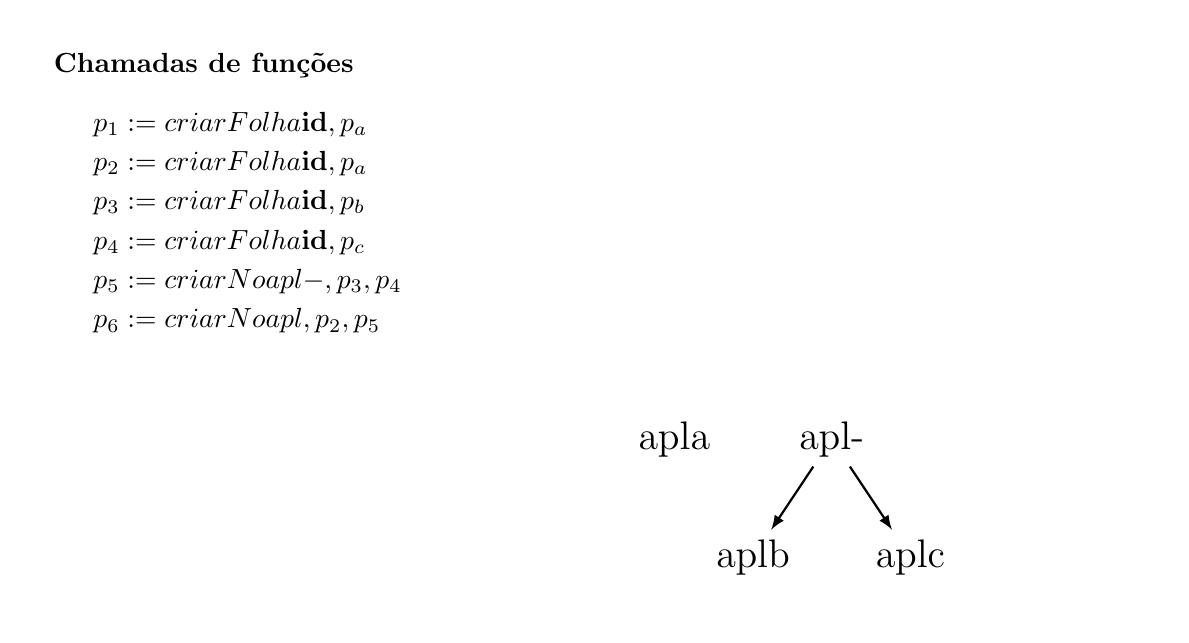
\begin{tikzpicture}
        \node[opacity=0] at (0, 0) { y };
        \node[opacity=0] at (14, 7) { t };

        \node[anchor=west] at (0, 6.75) { \textbf{Chamadas de funções} };
        \node[anchor=west] at (0.5, 6.0) { $p_1 := \Call{criarFolha}{\textbf{id}, p_a}$ };
        \node[anchor=west] at (0.5, 5.5) { $p_2 := \Call{criarFolha}{\textbf{id}, p_a}$ };
        \node[anchor=west] at (0.5, 5.0) { $p_3 := \Call{criarFolha}{\textbf{id}, p_b}$ };
        \node[anchor=west] at (0.5, 4.5) { $p_4 := \Call{criarFolha}{\textbf{id}, p_c}$ };
        \node[anchor=west] at (0.5, 4.0) { $p_5 := \Call{criarNo}{\code{apl}{-}, p_3, p_4}$ };
        \node[anchor=west] at (0.5, 3.5) { $p_6 := \Call{criarNo}{\code{apl}{×}, p_2, p_5}$ };
%        \node[anchor=west] at (0.5, 3.0) { $p_7 := \Call{criarFolha}{\textbf{id}, p_a}$ };
%        \node[anchor=west] at (0.5, 2.5) { $p_8 := \Call{criarFolha}{\textbf{id}, p_a}$ };
%        \node[anchor=west] at (0.5, 2.0) { $p_9 := \Call{criarFolha}{\textbf{id}, p_a}$ };
%        \node[anchor=west] at (0.5, 1.5) { $p_10 := \Call{criarFolha}{\textbf{id}, p_a}$ };
%        \node[anchor=west] at (0.5, 1.0) { $p_11 := \Call{criarFolha}{\textbf{id}, p_a}$ };
%        \node[anchor=west] at (0.5, 0.5) { $p_12 := \Call{criarFolha}{\textbf{id}, p_a}$ };
%        \node[anchor=west] at (0.5, 0.0) { $p_13 := \Call{criarFolha}{\textbf{id}, p_a}$ };

        \node (A) at (8, 2) { \Large \code{apl}{a} };
        \node (B) at (9, 0.5) { \Large \code{apl}{b} };
        \node (C) at (11, 0.5) { \Large \code{apl}{c} };
        \node (M) at (10, 2) { \Large \code{apl}{-} };

        \draw[thick,-latex] (M) to (B);
        \draw[thick,-latex] (M) to (C);

    \end{tikzpicture}

\end{frame}

\begin{frame}[fragile]{Criação do DAG para a expressão \code{apl}{a + a × (b - c) + (b - c) × d}}

    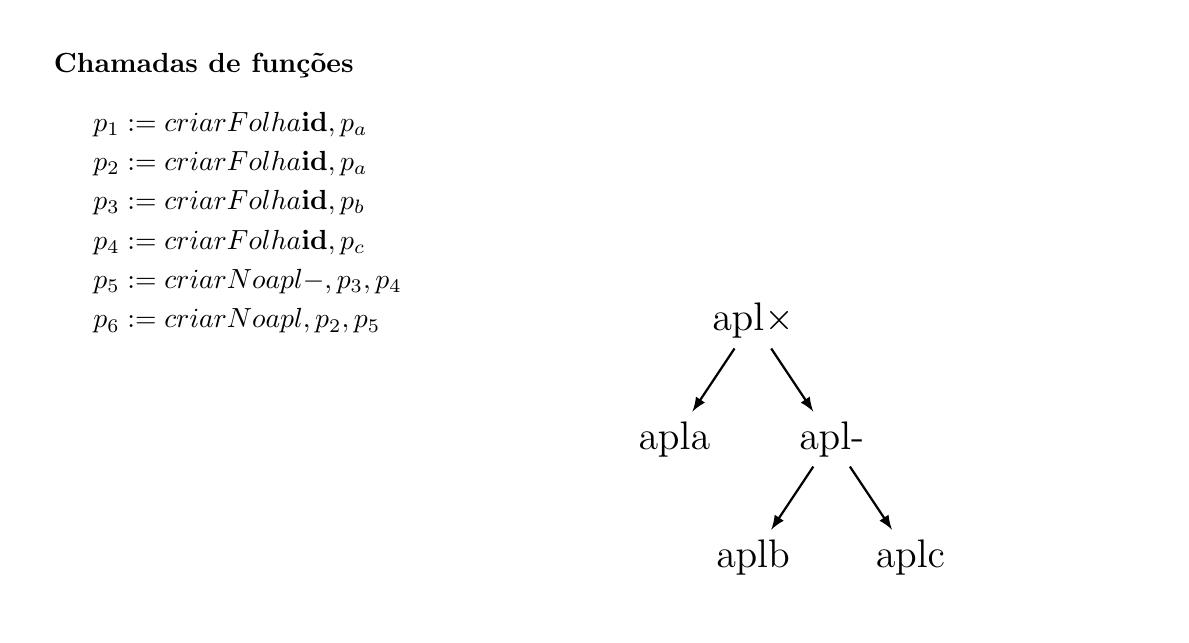
\begin{tikzpicture}
        \node[opacity=0] at (0, 0) { y };
        \node[opacity=0] at (14, 7) { t };

        \node[anchor=west] at (0, 6.75) { \textbf{Chamadas de funções} };
        \node[anchor=west] at (0.5, 6.0) { $p_1 := \Call{criarFolha}{\textbf{id}, p_a}$ };
        \node[anchor=west] at (0.5, 5.5) { $p_2 := \Call{criarFolha}{\textbf{id}, p_a}$ };
        \node[anchor=west] at (0.5, 5.0) { $p_3 := \Call{criarFolha}{\textbf{id}, p_b}$ };
        \node[anchor=west] at (0.5, 4.5) { $p_4 := \Call{criarFolha}{\textbf{id}, p_c}$ };
        \node[anchor=west] at (0.5, 4.0) { $p_5 := \Call{criarNo}{\code{apl}{-}, p_3, p_4}$ };
        \node[anchor=west] at (0.5, 3.5) { $p_6 := \Call{criarNo}{\code{apl}{×}, p_2, p_5}$ };
%        \node[anchor=west] at (0.5, 3.0) { $p_7 := \Call{criarFolha}{\textbf{id}, p_a}$ };
%        \node[anchor=west] at (0.5, 2.5) { $p_8 := \Call{criarFolha}{\textbf{id}, p_a}$ };
%        \node[anchor=west] at (0.5, 2.0) { $p_9 := \Call{criarFolha}{\textbf{id}, p_a}$ };
%        \node[anchor=west] at (0.5, 1.5) { $p_10 := \Call{criarFolha}{\textbf{id}, p_a}$ };
%        \node[anchor=west] at (0.5, 1.0) { $p_11 := \Call{criarFolha}{\textbf{id}, p_a}$ };
%        \node[anchor=west] at (0.5, 0.5) { $p_12 := \Call{criarFolha}{\textbf{id}, p_a}$ };
%        \node[anchor=west] at (0.5, 0.0) { $p_13 := \Call{criarFolha}{\textbf{id}, p_a}$ };

        \node (A) at (8, 2) { \Large \code{apl}{a} };
        \node (B) at (9, 0.5) { \Large \code{apl}{b} };
        \node (C) at (11, 0.5) { \Large \code{apl}{c} };
        \node (M) at (10, 2) { \Large \code{apl}{-} };
        \node (T1) at (9, 3.5) { \Large \code{apl}{×} };

        \draw[thick,-latex] (M) to (B);
        \draw[thick,-latex] (M) to (C);
        \draw[thick,-latex] (T1) to (M);
        \draw[thick,-latex] (T1) to (A);

    \end{tikzpicture}

\end{frame}

\begin{frame}[fragile]{Criação do DAG para a expressão \code{apl}{a + a × (b - c) + (b - c) × d}}

    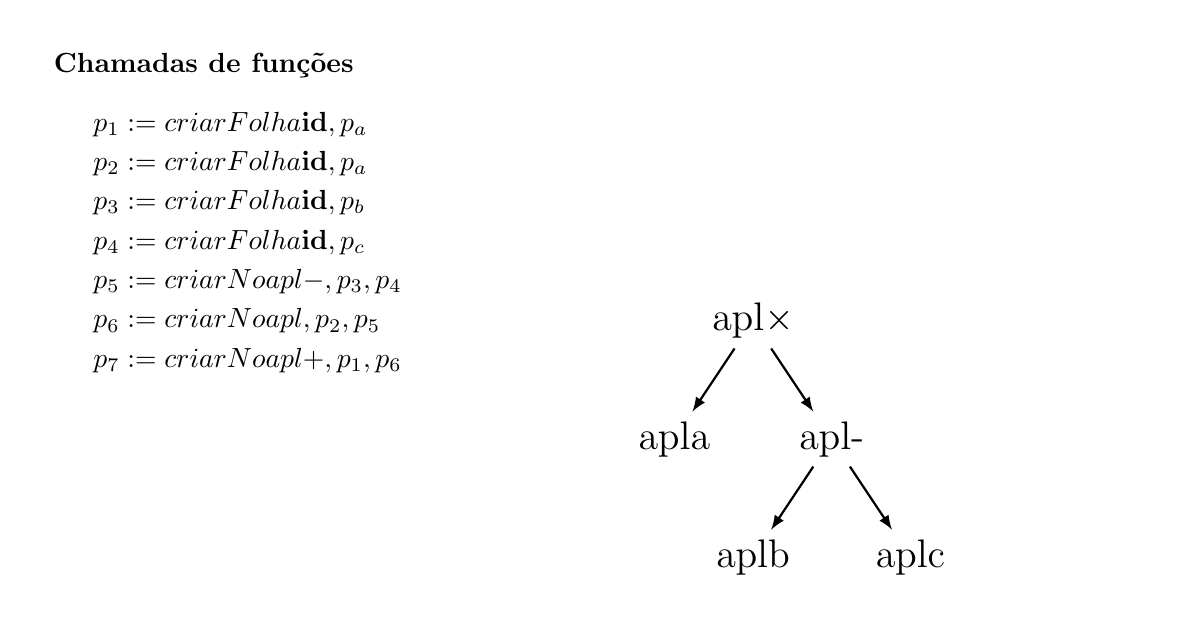
\begin{tikzpicture}
        \node[opacity=0] at (0, 0) { y };
        \node[opacity=0] at (14, 7) { t };

        \node[anchor=west] at (0, 6.75) { \textbf{Chamadas de funções} };
        \node[anchor=west] at (0.5, 6.0) { $p_1 := \Call{criarFolha}{\textbf{id}, p_a}$ };
        \node[anchor=west] at (0.5, 5.5) { $p_2 := \Call{criarFolha}{\textbf{id}, p_a}$ };
        \node[anchor=west] at (0.5, 5.0) { $p_3 := \Call{criarFolha}{\textbf{id}, p_b}$ };
        \node[anchor=west] at (0.5, 4.5) { $p_4 := \Call{criarFolha}{\textbf{id}, p_c}$ };
        \node[anchor=west] at (0.5, 4.0) { $p_5 := \Call{criarNo}{\code{apl}{-}, p_3, p_4}$ };
        \node[anchor=west] at (0.5, 3.5) { $p_6 := \Call{criarNo}{\code{apl}{×}, p_2, p_5}$ };
        \node[anchor=west] at (0.5, 3.0) { $p_7 := \Call{criarNo}{\code{apl}{+}, p_1, p_6}$ };
%        \node[anchor=west] at (0.5, 2.5) { $p_8 := \Call{criarFolha}{\textbf{id}, p_a}$ };
%        \node[anchor=west] at (0.5, 2.0) { $p_9 := \Call{criarFolha}{\textbf{id}, p_a}$ };
%        \node[anchor=west] at (0.5, 1.5) { $p_10 := \Call{criarFolha}{\textbf{id}, p_a}$ };
%        \node[anchor=west] at (0.5, 1.0) { $p_11 := \Call{criarFolha}{\textbf{id}, p_a}$ };
%        \node[anchor=west] at (0.5, 0.5) { $p_12 := \Call{criarFolha}{\textbf{id}, p_a}$ };
%        \node[anchor=west] at (0.5, 0.0) { $p_13 := \Call{criarFolha}{\textbf{id}, p_a}$ };

        \node (A) at (8, 2) { \Large \code{apl}{a} };
        \node (B) at (9, 0.5) { \Large \code{apl}{b} };
        \node (C) at (11, 0.5) { \Large \code{apl}{c} };
        \node (M) at (10, 2) { \Large \code{apl}{-} };
        \node (T1) at (9, 3.5) { \Large \code{apl}{×} };

        \draw[thick,-latex] (M) to (B);
        \draw[thick,-latex] (M) to (C);
        \draw[thick,-latex] (T1) to (M);
        \draw[thick,-latex] (T1) to (A);

    \end{tikzpicture}

\end{frame}

\begin{frame}[fragile]{Criação do DAG para a expressão \code{apl}{a + a × (b - c) + (b - c) × d}}

    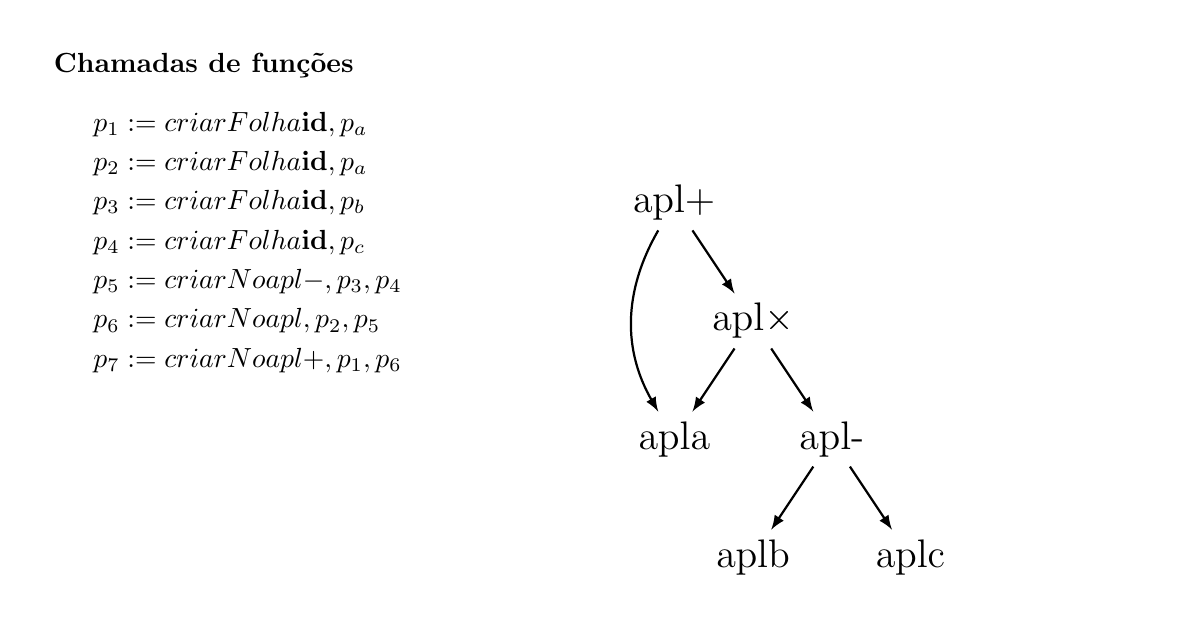
\begin{tikzpicture}
        \node[opacity=0] at (0, 0) { y };
        \node[opacity=0] at (14, 7) { t };

        \node[anchor=west] at (0, 6.75) { \textbf{Chamadas de funções} };
        \node[anchor=west] at (0.5, 6.0) { $p_1 := \Call{criarFolha}{\textbf{id}, p_a}$ };
        \node[anchor=west] at (0.5, 5.5) { $p_2 := \Call{criarFolha}{\textbf{id}, p_a}$ };
        \node[anchor=west] at (0.5, 5.0) { $p_3 := \Call{criarFolha}{\textbf{id}, p_b}$ };
        \node[anchor=west] at (0.5, 4.5) { $p_4 := \Call{criarFolha}{\textbf{id}, p_c}$ };
        \node[anchor=west] at (0.5, 4.0) { $p_5 := \Call{criarNo}{\code{apl}{-}, p_3, p_4}$ };
        \node[anchor=west] at (0.5, 3.5) { $p_6 := \Call{criarNo}{\code{apl}{×}, p_2, p_5}$ };
        \node[anchor=west] at (0.5, 3.0) { $p_7 := \Call{criarNo}{\code{apl}{+}, p_1, p_6}$ };
%        \node[anchor=west] at (0.5, 2.5) { $p_8 := \Call{criarFolha}{\textbf{id}, p_a}$ };
%        \node[anchor=west] at (0.5, 2.0) { $p_9 := \Call{criarFolha}{\textbf{id}, p_a}$ };
%        \node[anchor=west] at (0.5, 1.5) { $p_10 := \Call{criarFolha}{\textbf{id}, p_a}$ };
%        \node[anchor=west] at (0.5, 1.0) { $p_11 := \Call{criarFolha}{\textbf{id}, p_a}$ };
%        \node[anchor=west] at (0.5, 0.5) { $p_12 := \Call{criarFolha}{\textbf{id}, p_a}$ };
%        \node[anchor=west] at (0.5, 0.0) { $p_13 := \Call{criarFolha}{\textbf{id}, p_a}$ };

        \node (A) at (8, 2) { \Large \code{apl}{a} };
        \node (B) at (9, 0.5) { \Large \code{apl}{b} };
        \node (C) at (11, 0.5) { \Large \code{apl}{c} };
        \node (M) at (10, 2) { \Large \code{apl}{-} };
        \node (T1) at (9, 3.5) { \Large \code{apl}{×} };
        \node (P1) at (8, 5) { \Large \code{apl}{+} };

        \draw[thick,-latex] (M) to (B);
        \draw[thick,-latex] (M) to (C);
        \draw[thick,-latex] (T1) to (M);
        \draw[thick,-latex] (T1) to (A);
        \draw[thick,-latex] (P1) to [bend right] (A);
        \draw[thick,-latex] (P1) to (T1);

    \end{tikzpicture}

\end{frame}

\begin{frame}[fragile]{Criação do DAG para a expressão \code{apl}{a + a × (b - c) + (b - c) × d}}

    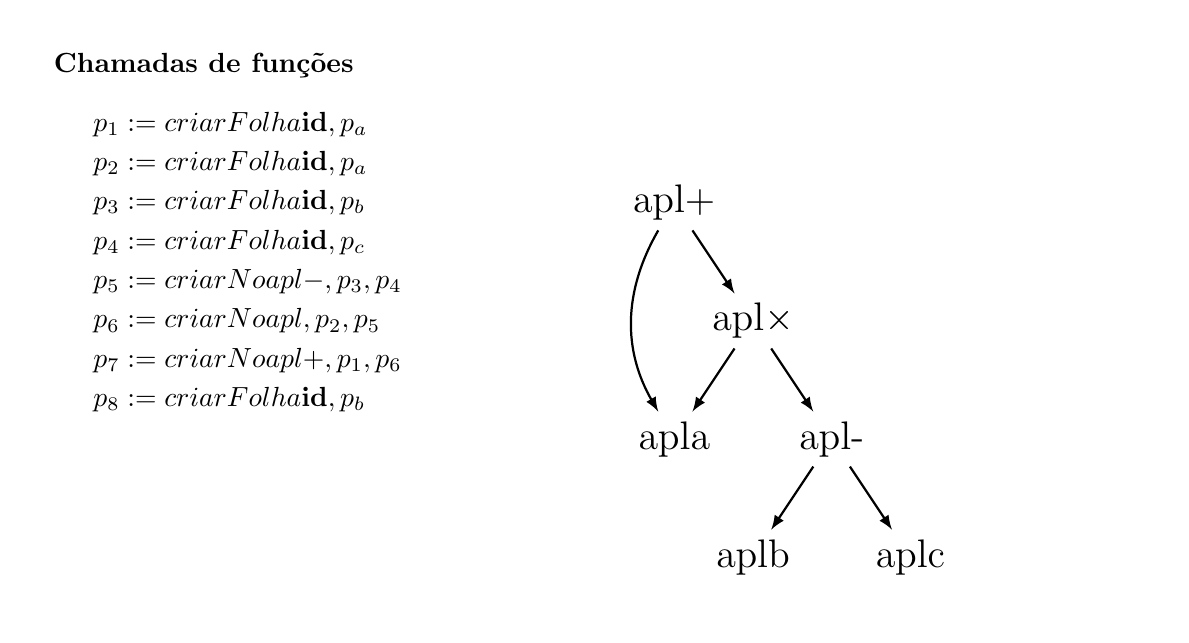
\begin{tikzpicture}
        \node[opacity=0] at (0, 0) { y };
        \node[opacity=0] at (14, 7) { t };

        \node[anchor=west] at (0, 6.75) { \textbf{Chamadas de funções} };
        \node[anchor=west] at (0.5, 6.0) { $p_1 := \Call{criarFolha}{\textbf{id}, p_a}$ };
        \node[anchor=west] at (0.5, 5.5) { $p_2 := \Call{criarFolha}{\textbf{id}, p_a}$ };
        \node[anchor=west] at (0.5, 5.0) { $p_3 := \Call{criarFolha}{\textbf{id}, p_b}$ };
        \node[anchor=west] at (0.5, 4.5) { $p_4 := \Call{criarFolha}{\textbf{id}, p_c}$ };
        \node[anchor=west] at (0.5, 4.0) { $p_5 := \Call{criarNo}{\code{apl}{-}, p_3, p_4}$ };
        \node[anchor=west] at (0.5, 3.5) { $p_6 := \Call{criarNo}{\code{apl}{×}, p_2, p_5}$ };
        \node[anchor=west] at (0.5, 3.0) { $p_7 := \Call{criarNo}{\code{apl}{+}, p_1, p_6}$ };
        \node[anchor=west] at (0.5, 2.5) { $p_8 := \Call{criarFolha}{\textbf{id}, p_b}$ };
%        \node[anchor=west] at (0.5, 2.0) { $p_9 := \Call{criarFolha}{\textbf{id}, p_a}$ };
%        \node[anchor=west] at (0.5, 1.5) { $p_10 := \Call{criarFolha}{\textbf{id}, p_a}$ };
%        \node[anchor=west] at (0.5, 1.0) { $p_11 := \Call{criarFolha}{\textbf{id}, p_a}$ };
%        \node[anchor=west] at (0.5, 0.5) { $p_12 := \Call{criarFolha}{\textbf{id}, p_a}$ };
%        \node[anchor=west] at (0.5, 0.0) { $p_13 := \Call{criarFolha}{\textbf{id}, p_a}$ };

        \node (A) at (8, 2) { \Large \code{apl}{a} };
        \node (B) at (9, 0.5) { \Large \code{apl}{b} };
        \node (C) at (11, 0.5) { \Large \code{apl}{c} };
        \node (M) at (10, 2) { \Large \code{apl}{-} };
        \node (T1) at (9, 3.5) { \Large \code{apl}{×} };
        \node (P1) at (8, 5) { \Large \code{apl}{+} };

        \draw[thick,-latex] (M) to (B);
        \draw[thick,-latex] (M) to (C);
        \draw[thick,-latex] (T1) to (M);
        \draw[thick,-latex] (T1) to (A);
        \draw[thick,-latex] (P1) to [bend right] (A);
        \draw[thick,-latex] (P1) to (T1);

    \end{tikzpicture}

\end{frame}

\begin{frame}[fragile]{Criação do DAG para a expressão \code{apl}{a + a × (b - c) + (b - c) × d}}

    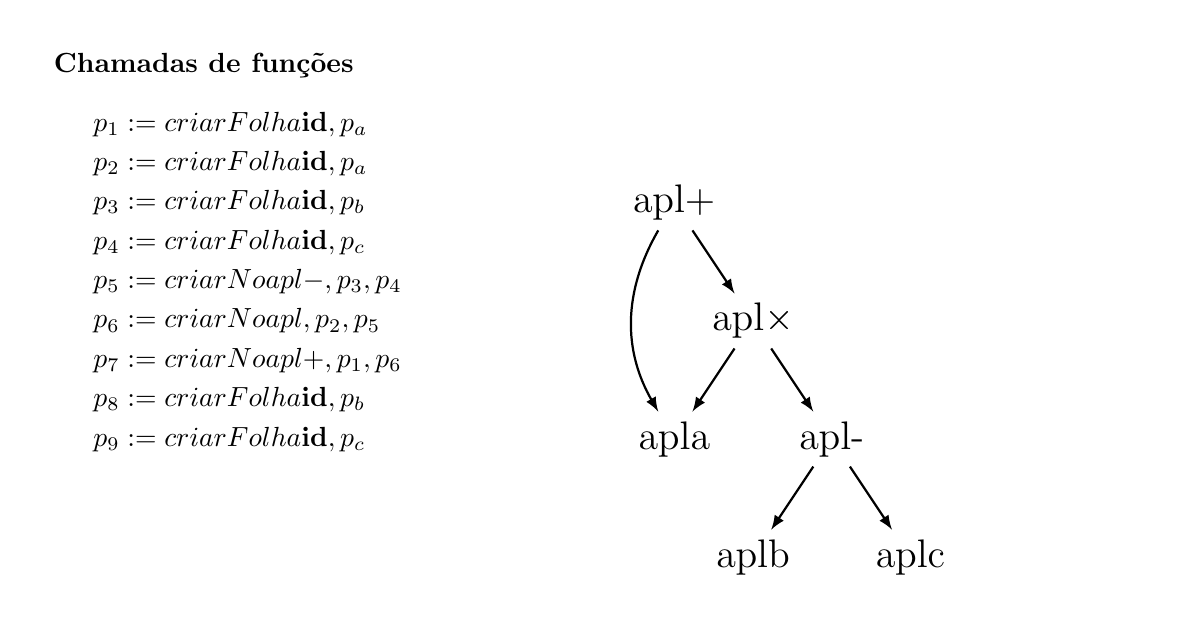
\begin{tikzpicture}
        \node[opacity=0] at (0, 0) { y };
        \node[opacity=0] at (14, 7) { t };

        \node[anchor=west] at (0, 6.75) { \textbf{Chamadas de funções} };
        \node[anchor=west] at (0.5, 6.0) { $p_1 := \Call{criarFolha}{\textbf{id}, p_a}$ };
        \node[anchor=west] at (0.5, 5.5) { $p_2 := \Call{criarFolha}{\textbf{id}, p_a}$ };
        \node[anchor=west] at (0.5, 5.0) { $p_3 := \Call{criarFolha}{\textbf{id}, p_b}$ };
        \node[anchor=west] at (0.5, 4.5) { $p_4 := \Call{criarFolha}{\textbf{id}, p_c}$ };
        \node[anchor=west] at (0.5, 4.0) { $p_5 := \Call{criarNo}{\code{apl}{-}, p_3, p_4}$ };
        \node[anchor=west] at (0.5, 3.5) { $p_6 := \Call{criarNo}{\code{apl}{×}, p_2, p_5}$ };
        \node[anchor=west] at (0.5, 3.0) { $p_7 := \Call{criarNo}{\code{apl}{+}, p_1, p_6}$ };
        \node[anchor=west] at (0.5, 2.5) { $p_8 := \Call{criarFolha}{\textbf{id}, p_b}$ };
        \node[anchor=west] at (0.5, 2.0) { $p_9 := \Call{criarFolha}{\textbf{id}, p_c}$ };
%        \node[anchor=west] at (0.5, 1.5) { $p_10 := \Call{criarFolha}{\textbf{id}, p_a}$ };
%        \node[anchor=west] at (0.5, 1.0) { $p_11 := \Call{criarFolha}{\textbf{id}, p_a}$ };
%        \node[anchor=west] at (0.5, 0.5) { $p_12 := \Call{criarFolha}{\textbf{id}, p_a}$ };
%        \node[anchor=west] at (0.5, 0.0) { $p_13 := \Call{criarFolha}{\textbf{id}, p_a}$ };

        \node (A) at (8, 2) { \Large \code{apl}{a} };
        \node (B) at (9, 0.5) { \Large \code{apl}{b} };
        \node (C) at (11, 0.5) { \Large \code{apl}{c} };
        \node (M) at (10, 2) { \Large \code{apl}{-} };
        \node (T1) at (9, 3.5) { \Large \code{apl}{×} };
        \node (P1) at (8, 5) { \Large \code{apl}{+} };

        \draw[thick,-latex] (M) to (B);
        \draw[thick,-latex] (M) to (C);
        \draw[thick,-latex] (T1) to (M);
        \draw[thick,-latex] (T1) to (A);
        \draw[thick,-latex] (P1) to [bend right] (A);
        \draw[thick,-latex] (P1) to (T1);

    \end{tikzpicture}

\end{frame}

\begin{frame}[fragile]{Criação do DAG para a expressão \code{apl}{a + a × (b - c) + (b - c) × d}}

    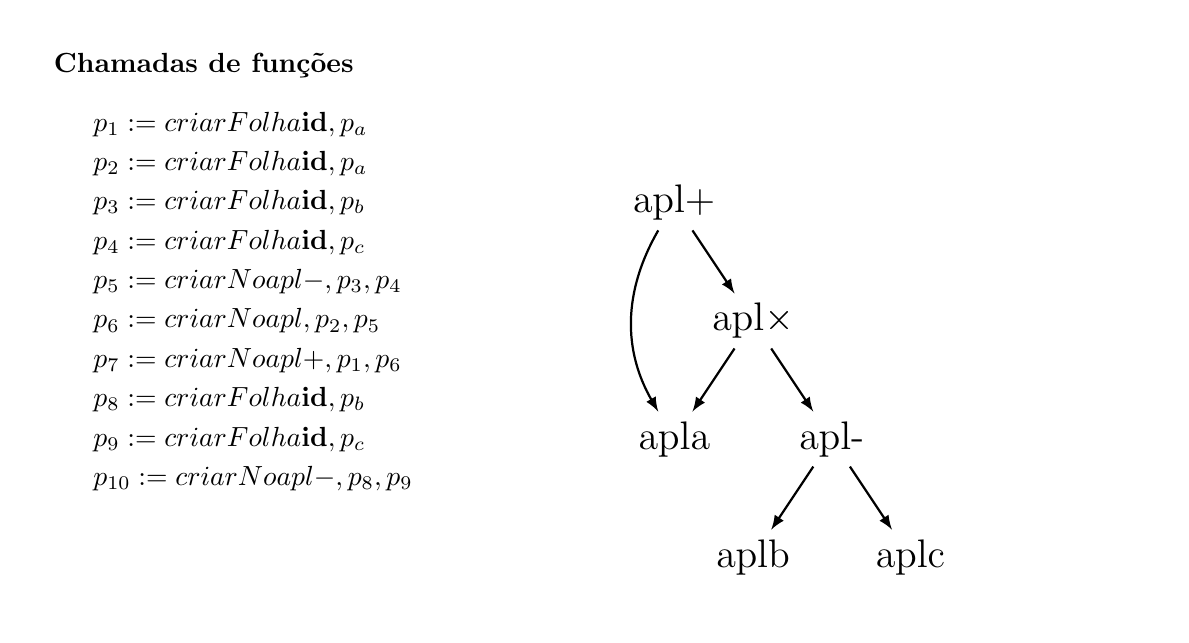
\begin{tikzpicture}
        \node[opacity=0] at (0, 0) { y };
        \node[opacity=0] at (14, 7) { t };

        \node[anchor=west] at (0, 6.75) { \textbf{Chamadas de funções} };
        \node[anchor=west] at (0.5, 6.0) { $p_1 := \Call{criarFolha}{\textbf{id}, p_a}$ };
        \node[anchor=west] at (0.5, 5.5) { $p_2 := \Call{criarFolha}{\textbf{id}, p_a}$ };
        \node[anchor=west] at (0.5, 5.0) { $p_3 := \Call{criarFolha}{\textbf{id}, p_b}$ };
        \node[anchor=west] at (0.5, 4.5) { $p_4 := \Call{criarFolha}{\textbf{id}, p_c}$ };
        \node[anchor=west] at (0.5, 4.0) { $p_5 := \Call{criarNo}{\code{apl}{-}, p_3, p_4}$ };
        \node[anchor=west] at (0.5, 3.5) { $p_6 := \Call{criarNo}{\code{apl}{×}, p_2, p_5}$ };
        \node[anchor=west] at (0.5, 3.0) { $p_7 := \Call{criarNo}{\code{apl}{+}, p_1, p_6}$ };
        \node[anchor=west] at (0.5, 2.5) { $p_8 := \Call{criarFolha}{\textbf{id}, p_b}$ };
        \node[anchor=west] at (0.5, 2.0) { $p_9 := \Call{criarFolha}{\textbf{id}, p_c}$ };
        \node[anchor=west] at (0.5, 1.5) { $p_{10} := \Call{criarNo}{\code{apl}{-}, p_8, p_9}$ };
%        \node[anchor=west] at (0.5, 1.0) { $p_11 := \Call{criarFolha}{\textbf{id}, p_a}$ };
%        \node[anchor=west] at (0.5, 0.5) { $p_12 := \Call{criarFolha}{\textbf{id}, p_a}$ };
%        \node[anchor=west] at (0.5, 0.0) { $p_13 := \Call{criarFolha}{\textbf{id}, p_a}$ };

        \node (A) at (8, 2) { \Large \code{apl}{a} };
        \node (B) at (9, 0.5) { \Large \code{apl}{b} };
        \node (C) at (11, 0.5) { \Large \code{apl}{c} };
        \node (M) at (10, 2) { \Large \code{apl}{-} };
        \node (T1) at (9, 3.5) { \Large \code{apl}{×} };
        \node (P1) at (8, 5) { \Large \code{apl}{+} };

        \draw[thick,-latex] (M) to (B);
        \draw[thick,-latex] (M) to (C);
        \draw[thick,-latex] (T1) to (M);
        \draw[thick,-latex] (T1) to (A);
        \draw[thick,-latex] (P1) to [bend right] (A);
        \draw[thick,-latex] (P1) to (T1);

    \end{tikzpicture}

\end{frame}

\begin{frame}[fragile]{Criação do DAG para a expressão \code{apl}{a + a × (b - c) + (b - c) × d}}

    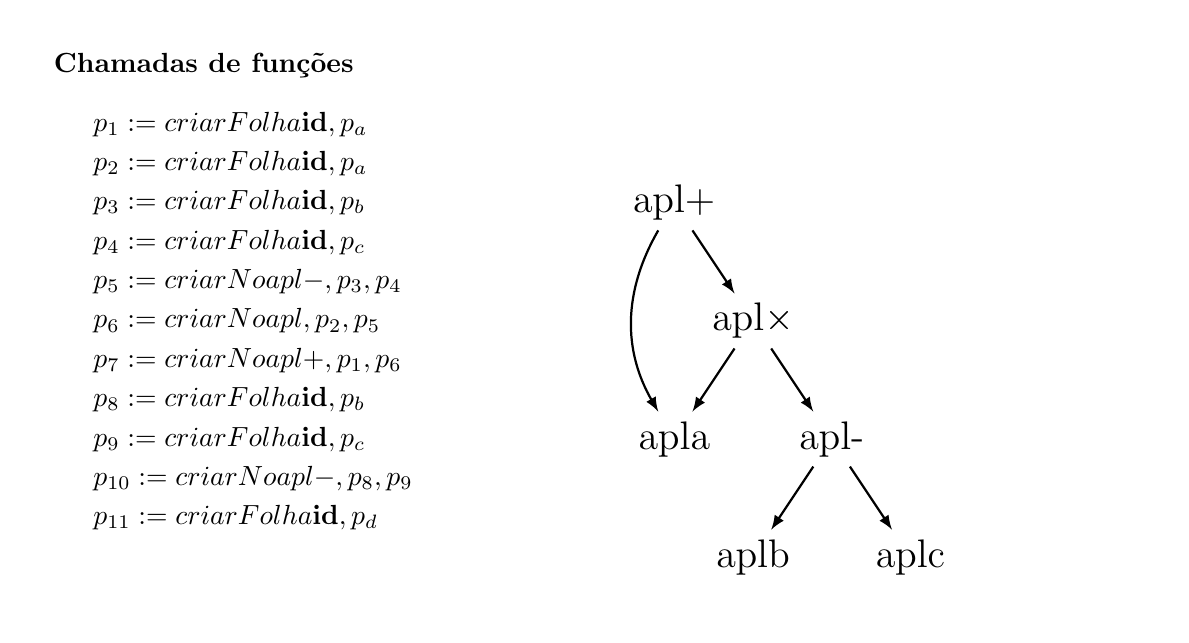
\begin{tikzpicture}
        \node[opacity=0] at (0, 0) { y };
        \node[opacity=0] at (14, 7) { t };

        \node[anchor=west] at (0, 6.75) { \textbf{Chamadas de funções} };
        \node[anchor=west] at (0.5, 6.0) { $p_1 := \Call{criarFolha}{\textbf{id}, p_a}$ };
        \node[anchor=west] at (0.5, 5.5) { $p_2 := \Call{criarFolha}{\textbf{id}, p_a}$ };
        \node[anchor=west] at (0.5, 5.0) { $p_3 := \Call{criarFolha}{\textbf{id}, p_b}$ };
        \node[anchor=west] at (0.5, 4.5) { $p_4 := \Call{criarFolha}{\textbf{id}, p_c}$ };
        \node[anchor=west] at (0.5, 4.0) { $p_5 := \Call{criarNo}{\code{apl}{-}, p_3, p_4}$ };
        \node[anchor=west] at (0.5, 3.5) { $p_6 := \Call{criarNo}{\code{apl}{×}, p_2, p_5}$ };
        \node[anchor=west] at (0.5, 3.0) { $p_7 := \Call{criarNo}{\code{apl}{+}, p_1, p_6}$ };
        \node[anchor=west] at (0.5, 2.5) { $p_8 := \Call{criarFolha}{\textbf{id}, p_b}$ };
        \node[anchor=west] at (0.5, 2.0) { $p_9 := \Call{criarFolha}{\textbf{id}, p_c}$ };
        \node[anchor=west] at (0.5, 1.5) { $p_{10} := \Call{criarNo}{\code{apl}{-}, p_8, p_9}$ };
        \node[anchor=west] at (0.5, 1.0) { $p_{11} := \Call{criarFolha}{\textbf{id}, p_d}$ };
%        \node[anchor=west] at (0.5, 0.5) { $p_12 := \Call{criarFolha}{\textbf{id}, p_a}$ };
%        \node[anchor=west] at (0.5, 0.0) { $p_13 := \Call{criarFolha}{\textbf{id}, p_a}$ };

        \node (A) at (8, 2) { \Large \code{apl}{a} };
        \node (B) at (9, 0.5) { \Large \code{apl}{b} };
        \node (C) at (11, 0.5) { \Large \code{apl}{c} };
        \node (M) at (10, 2) { \Large \code{apl}{-} };
        \node (T1) at (9, 3.5) { \Large \code{apl}{×} };
        \node (P1) at (8, 5) { \Large \code{apl}{+} };

        \draw[thick,-latex] (M) to (B);
        \draw[thick,-latex] (M) to (C);
        \draw[thick,-latex] (T1) to (M);
        \draw[thick,-latex] (T1) to (A);
        \draw[thick,-latex] (P1) to [bend right] (A);
        \draw[thick,-latex] (P1) to (T1);

    \end{tikzpicture}

\end{frame}

\begin{frame}[fragile]{Criação do DAG para a expressão \code{apl}{a + a × (b - c) + (b - c) × d}}

    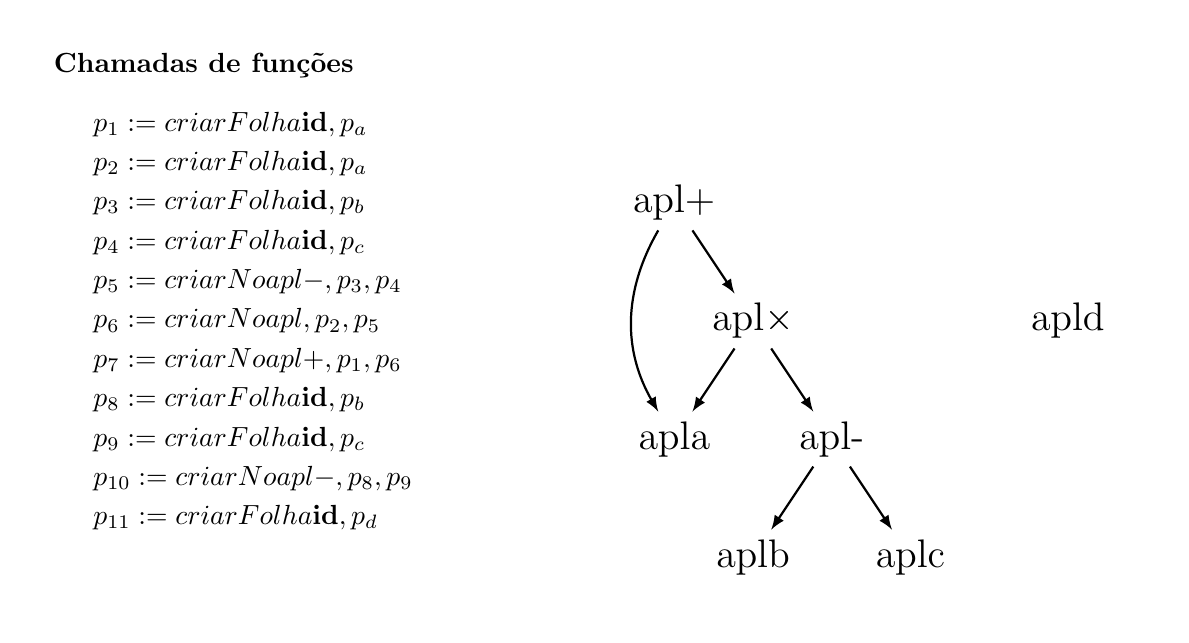
\begin{tikzpicture}
        \node[opacity=0] at (0, 0) { y };
        \node[opacity=0] at (14, 7) { t };

        \node[anchor=west] at (0, 6.75) { \textbf{Chamadas de funções} };
        \node[anchor=west] at (0.5, 6.0) { $p_1 := \Call{criarFolha}{\textbf{id}, p_a}$ };
        \node[anchor=west] at (0.5, 5.5) { $p_2 := \Call{criarFolha}{\textbf{id}, p_a}$ };
        \node[anchor=west] at (0.5, 5.0) { $p_3 := \Call{criarFolha}{\textbf{id}, p_b}$ };
        \node[anchor=west] at (0.5, 4.5) { $p_4 := \Call{criarFolha}{\textbf{id}, p_c}$ };
        \node[anchor=west] at (0.5, 4.0) { $p_5 := \Call{criarNo}{\code{apl}{-}, p_3, p_4}$ };
        \node[anchor=west] at (0.5, 3.5) { $p_6 := \Call{criarNo}{\code{apl}{×}, p_2, p_5}$ };
        \node[anchor=west] at (0.5, 3.0) { $p_7 := \Call{criarNo}{\code{apl}{+}, p_1, p_6}$ };
        \node[anchor=west] at (0.5, 2.5) { $p_8 := \Call{criarFolha}{\textbf{id}, p_b}$ };
        \node[anchor=west] at (0.5, 2.0) { $p_9 := \Call{criarFolha}{\textbf{id}, p_c}$ };
        \node[anchor=west] at (0.5, 1.5) { $p_{10} := \Call{criarNo}{\code{apl}{-}, p_8, p_9}$ };
        \node[anchor=west] at (0.5, 1.0) { $p_{11} := \Call{criarFolha}{\textbf{id}, p_d}$ };
%        \node[anchor=west] at (0.5, 0.5) { $p_12 := \Call{criarFolha}{\textbf{id}, p_a}$ };
%        \node[anchor=west] at (0.5, 0.0) { $p_13 := \Call{criarFolha}{\textbf{id}, p_a}$ };

        \node (A) at (8, 2) { \Large \code{apl}{a} };
        \node (B) at (9, 0.5) { \Large \code{apl}{b} };
        \node (C) at (11, 0.5) { \Large \code{apl}{c} };
        \node (M) at (10, 2) { \Large \code{apl}{-} };
        \node (T1) at (9, 3.5) { \Large \code{apl}{×} };
        \node (P1) at (8, 5) { \Large \code{apl}{+} };
        \node (D) at (13, 3.5) { \Large \code{apl}{d} };

        \draw[thick,-latex] (M) to (B);
        \draw[thick,-latex] (M) to (C);
        \draw[thick,-latex] (T1) to (M);
        \draw[thick,-latex] (T1) to (A);
        \draw[thick,-latex] (P1) to [bend right] (A);
        \draw[thick,-latex] (P1) to (T1);

    \end{tikzpicture}

\end{frame}

\begin{frame}[fragile]{Criação do DAG para a expressão \code{apl}{a + a × (b - c) + (b - c) × d}}

    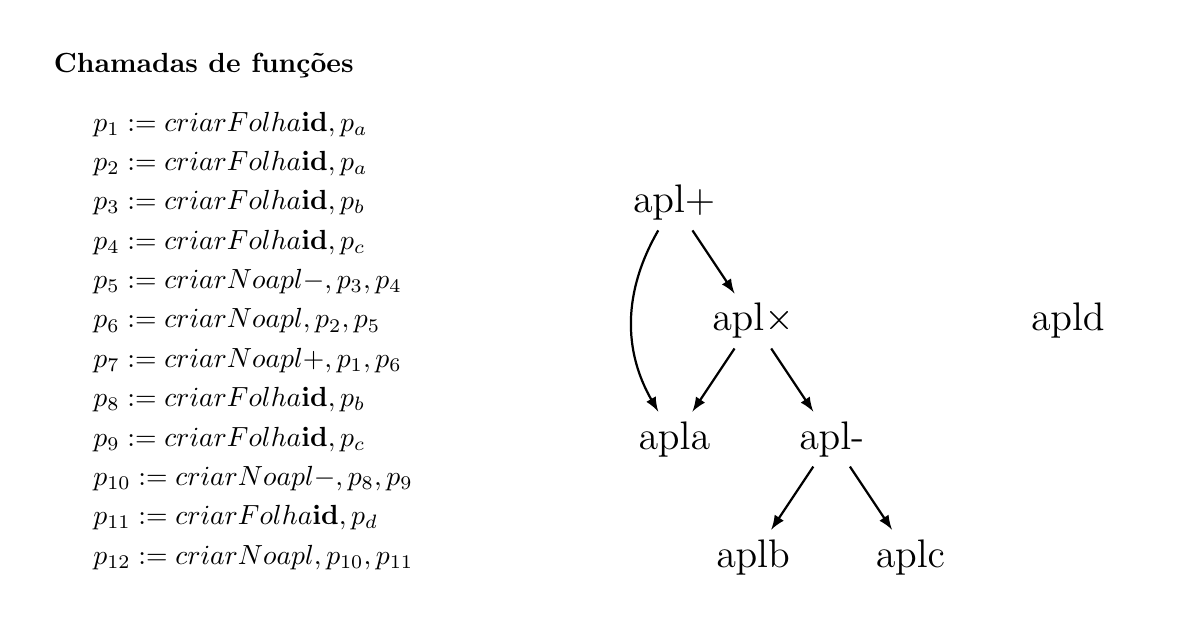
\begin{tikzpicture}
        \node[opacity=0] at (0, 0) { y };
        \node[opacity=0] at (14, 7) { t };

        \node[anchor=west] at (0, 6.75) { \textbf{Chamadas de funções} };
        \node[anchor=west] at (0.5, 6.0) { $p_1 := \Call{criarFolha}{\textbf{id}, p_a}$ };
        \node[anchor=west] at (0.5, 5.5) { $p_2 := \Call{criarFolha}{\textbf{id}, p_a}$ };
        \node[anchor=west] at (0.5, 5.0) { $p_3 := \Call{criarFolha}{\textbf{id}, p_b}$ };
        \node[anchor=west] at (0.5, 4.5) { $p_4 := \Call{criarFolha}{\textbf{id}, p_c}$ };
        \node[anchor=west] at (0.5, 4.0) { $p_5 := \Call{criarNo}{\code{apl}{-}, p_3, p_4}$ };
        \node[anchor=west] at (0.5, 3.5) { $p_6 := \Call{criarNo}{\code{apl}{×}, p_2, p_5}$ };
        \node[anchor=west] at (0.5, 3.0) { $p_7 := \Call{criarNo}{\code{apl}{+}, p_1, p_6}$ };
        \node[anchor=west] at (0.5, 2.5) { $p_8 := \Call{criarFolha}{\textbf{id}, p_b}$ };
        \node[anchor=west] at (0.5, 2.0) { $p_9 := \Call{criarFolha}{\textbf{id}, p_c}$ };
        \node[anchor=west] at (0.5, 1.5) { $p_{10} := \Call{criarNo}{\code{apl}{-}, p_8, p_9}$ };
        \node[anchor=west] at (0.5, 1.0) { $p_{11} := \Call{criarFolha}{\textbf{id}, p_d}$ };
        \node[anchor=west] at (0.5, 0.5) { $p_{12} := \Call{criarNo}{\code{apl}{×}, p_{10}, p_{11}}$ };
%        \node[anchor=west] at (0.5, 0.0) { $p_13 := \Call{criarFolha}{\textbf{id}, p_a}$ };

        \node (A) at (8, 2) { \Large \code{apl}{a} };
        \node (B) at (9, 0.5) { \Large \code{apl}{b} };
        \node (C) at (11, 0.5) { \Large \code{apl}{c} };
        \node (M) at (10, 2) { \Large \code{apl}{-} };
        \node (T1) at (9, 3.5) { \Large \code{apl}{×} };
        \node (P1) at (8, 5) { \Large \code{apl}{+} };
        \node (D) at (13, 3.5) { \Large \code{apl}{d} };

        \draw[thick,-latex] (M) to (B);
        \draw[thick,-latex] (M) to (C);
        \draw[thick,-latex] (T1) to (M);
        \draw[thick,-latex] (T1) to (A);
        \draw[thick,-latex] (P1) to [bend right] (A);
        \draw[thick,-latex] (P1) to (T1);

    \end{tikzpicture}

\end{frame}

\begin{frame}[fragile]{Criação do DAG para a expressão \code{apl}{a + a × (b - c) + (b - c) × d}}

    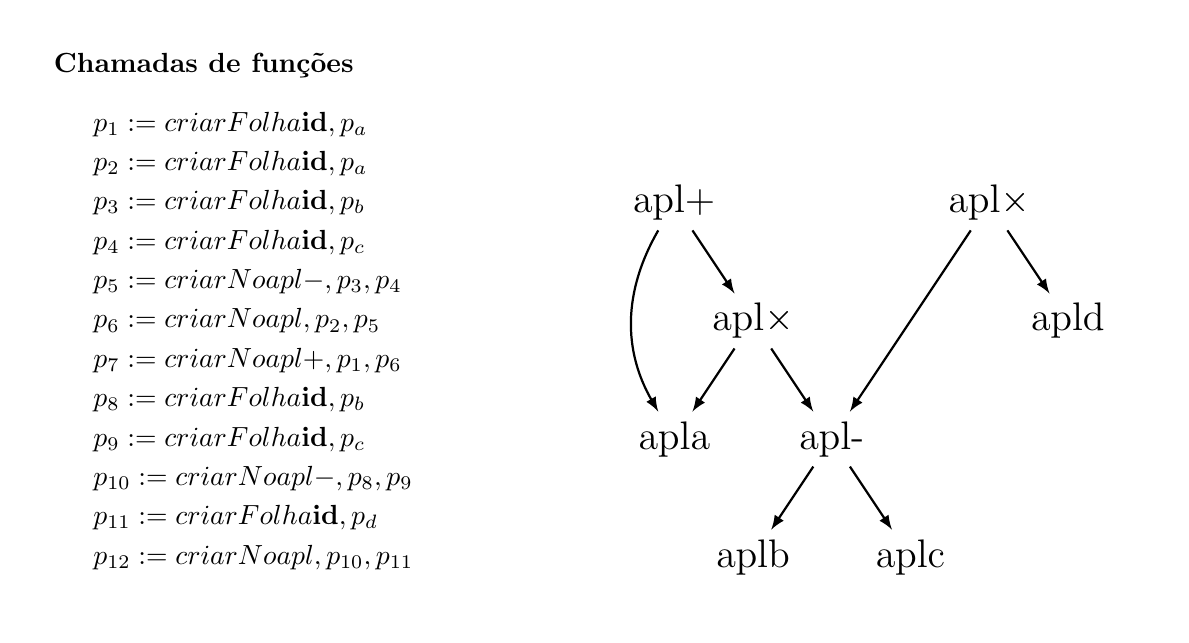
\begin{tikzpicture}
        \node[opacity=0] at (0, 0) { y };
        \node[opacity=0] at (14, 7) { t };

        \node[anchor=west] at (0, 6.75) { \textbf{Chamadas de funções} };
        \node[anchor=west] at (0.5, 6.0) { $p_1 := \Call{criarFolha}{\textbf{id}, p_a}$ };
        \node[anchor=west] at (0.5, 5.5) { $p_2 := \Call{criarFolha}{\textbf{id}, p_a}$ };
        \node[anchor=west] at (0.5, 5.0) { $p_3 := \Call{criarFolha}{\textbf{id}, p_b}$ };
        \node[anchor=west] at (0.5, 4.5) { $p_4 := \Call{criarFolha}{\textbf{id}, p_c}$ };
        \node[anchor=west] at (0.5, 4.0) { $p_5 := \Call{criarNo}{\code{apl}{-}, p_3, p_4}$ };
        \node[anchor=west] at (0.5, 3.5) { $p_6 := \Call{criarNo}{\code{apl}{×}, p_2, p_5}$ };
        \node[anchor=west] at (0.5, 3.0) { $p_7 := \Call{criarNo}{\code{apl}{+}, p_1, p_6}$ };
        \node[anchor=west] at (0.5, 2.5) { $p_8 := \Call{criarFolha}{\textbf{id}, p_b}$ };
        \node[anchor=west] at (0.5, 2.0) { $p_9 := \Call{criarFolha}{\textbf{id}, p_c}$ };
        \node[anchor=west] at (0.5, 1.5) { $p_{10} := \Call{criarNo}{\code{apl}{-}, p_8, p_9}$ };
        \node[anchor=west] at (0.5, 1.0) { $p_{11} := \Call{criarFolha}{\textbf{id}, p_d}$ };
        \node[anchor=west] at (0.5, 0.5) { $p_{12} := \Call{criarNo}{\code{apl}{×}, p_{10}, p_{11}}$ };
%        \node[anchor=west] at (0.5, 0.0) { $p_13 := \Call{criarFolha}{\textbf{id}, p_a}$ };

        \node (A) at (8, 2) { \Large \code{apl}{a} };
        \node (B) at (9, 0.5) { \Large \code{apl}{b} };
        \node (C) at (11, 0.5) { \Large \code{apl}{c} };
        \node (M) at (10, 2) { \Large \code{apl}{-} };
        \node (T1) at (9, 3.5) { \Large \code{apl}{×} };
        \node (P1) at (8, 5) { \Large \code{apl}{+} };
        \node (D) at (13, 3.5) { \Large \code{apl}{d} };
        \node (T2) at (12, 5) { \Large \code{apl}{×} };

        \draw[thick,-latex] (M) to (B);
        \draw[thick,-latex] (M) to (C);
        \draw[thick,-latex] (T1) to (M);
        \draw[thick,-latex] (T1) to (A);
        \draw[thick,-latex] (P1) to [bend right] (A);
        \draw[thick,-latex] (P1) to (T1);
        \draw[thick,-latex] (T2) to (D);
        \draw[thick,-latex] (T2) to (M);

    \end{tikzpicture}

\end{frame}

\begin{frame}[fragile]{Criação do DAG para a expressão \code{apl}{a + a × (b - c) + (b - c) × d}}

    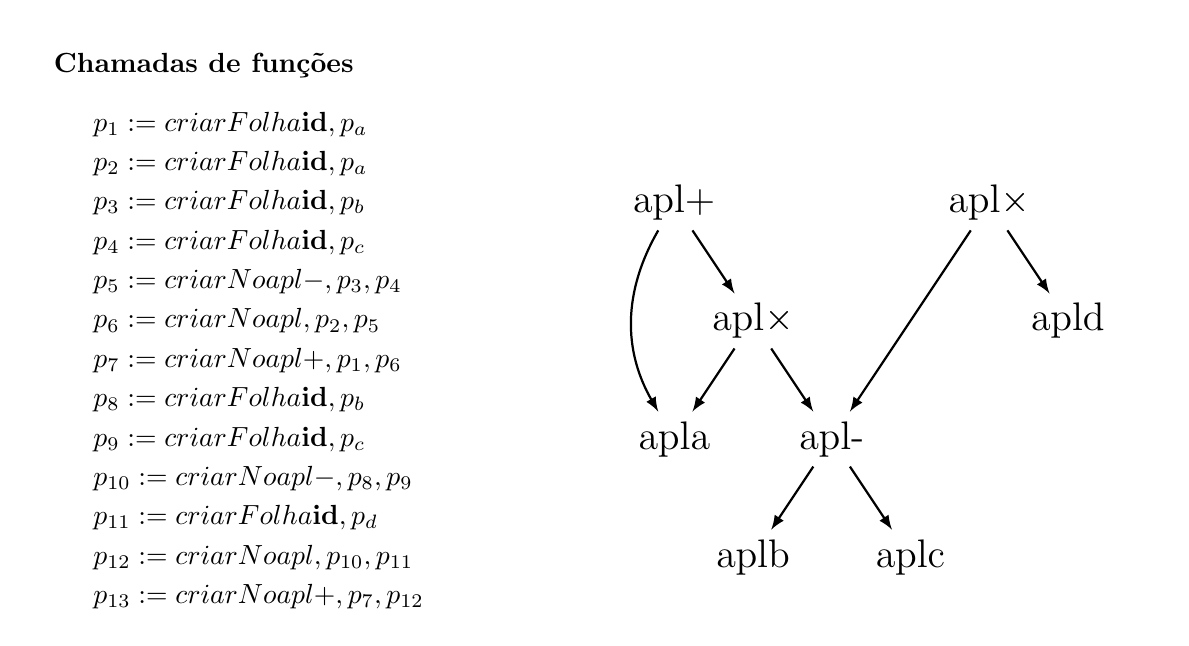
\begin{tikzpicture}
        \node[opacity=0] at (0, 0) { y };
        \node[opacity=0] at (14, 7) { t };

        \node[anchor=west] at (0, 6.75) { \textbf{Chamadas de funções} };
        \node[anchor=west] at (0.5, 6.0) { $p_1 := \Call{criarFolha}{\textbf{id}, p_a}$ };
        \node[anchor=west] at (0.5, 5.5) { $p_2 := \Call{criarFolha}{\textbf{id}, p_a}$ };
        \node[anchor=west] at (0.5, 5.0) { $p_3 := \Call{criarFolha}{\textbf{id}, p_b}$ };
        \node[anchor=west] at (0.5, 4.5) { $p_4 := \Call{criarFolha}{\textbf{id}, p_c}$ };
        \node[anchor=west] at (0.5, 4.0) { $p_5 := \Call{criarNo}{\code{apl}{-}, p_3, p_4}$ };
        \node[anchor=west] at (0.5, 3.5) { $p_6 := \Call{criarNo}{\code{apl}{×}, p_2, p_5}$ };
        \node[anchor=west] at (0.5, 3.0) { $p_7 := \Call{criarNo}{\code{apl}{+}, p_1, p_6}$ };
        \node[anchor=west] at (0.5, 2.5) { $p_8 := \Call{criarFolha}{\textbf{id}, p_b}$ };
        \node[anchor=west] at (0.5, 2.0) { $p_9 := \Call{criarFolha}{\textbf{id}, p_c}$ };
        \node[anchor=west] at (0.5, 1.5) { $p_{10} := \Call{criarNo}{\code{apl}{-}, p_8, p_9}$ };
        \node[anchor=west] at (0.5, 1.0) { $p_{11} := \Call{criarFolha}{\textbf{id}, p_d}$ };
        \node[anchor=west] at (0.5, 0.5) { $p_{12} := \Call{criarNo}{\code{apl}{×}, p_{10}, p_{11}}$ };
        \node[anchor=west] at (0.5, 0.0) { $p_{13} := \Call{criarNo}{\code{apl}{+}, p_{7}, p_{12}}$ };

        \node (A) at (8, 2) { \Large \code{apl}{a} };
        \node (B) at (9, 0.5) { \Large \code{apl}{b} };
        \node (C) at (11, 0.5) { \Large \code{apl}{c} };
        \node (M) at (10, 2) { \Large \code{apl}{-} };
        \node (T1) at (9, 3.5) { \Large \code{apl}{×} };
        \node (P1) at (8, 5) { \Large \code{apl}{+} };
        \node (D) at (13, 3.5) { \Large \code{apl}{d} };
        \node (T2) at (12, 5) { \Large \code{apl}{×} };

        \draw[thick,-latex] (M) to (B);
        \draw[thick,-latex] (M) to (C);
        \draw[thick,-latex] (T1) to (M);
        \draw[thick,-latex] (T1) to (A);
        \draw[thick,-latex] (P1) to [bend right] (A);
        \draw[thick,-latex] (P1) to (T1);
        \draw[thick,-latex] (T2) to (D);
        \draw[thick,-latex] (T2) to (M);

    \end{tikzpicture}

\end{frame}

\begin{frame}[fragile]{Criação do DAG para a expressão \code{apl}{a + a × (b - c) + (b - c) × d}}

    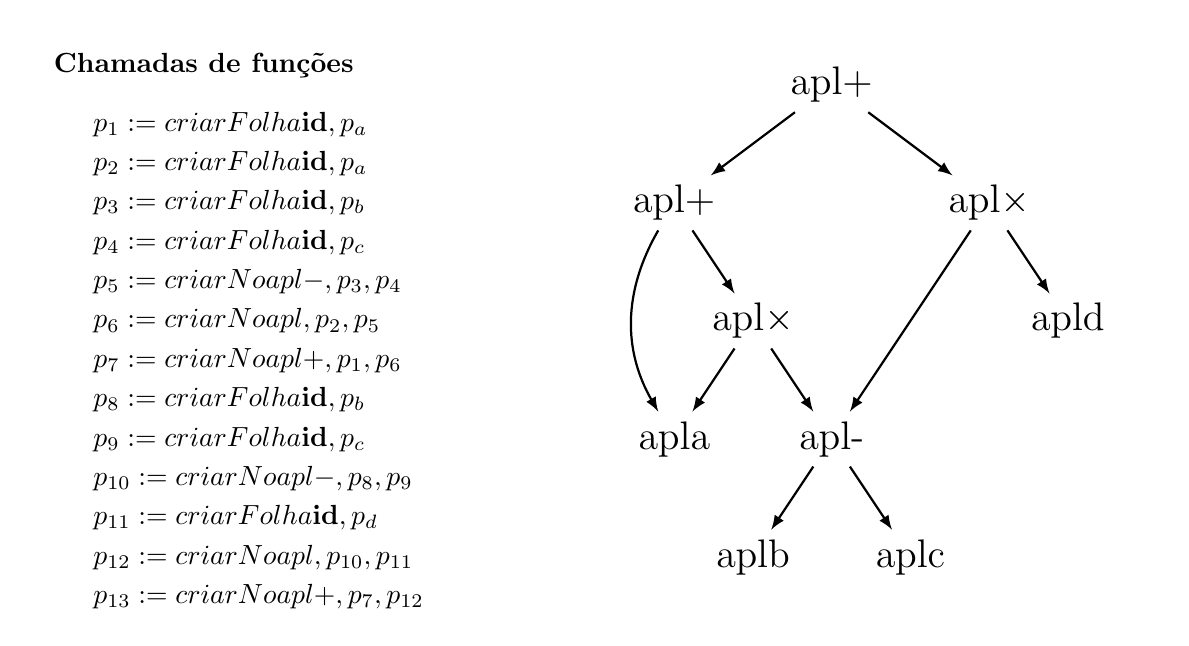
\begin{tikzpicture}
        \node[opacity=0] at (0, 0) { y };
        \node[opacity=0] at (14, 7) { t };

        \node[anchor=west] at (0, 6.75) { \textbf{Chamadas de funções} };
        \node[anchor=west] at (0.5, 6.0) { $p_1 := \Call{criarFolha}{\textbf{id}, p_a}$ };
        \node[anchor=west] at (0.5, 5.5) { $p_2 := \Call{criarFolha}{\textbf{id}, p_a}$ };
        \node[anchor=west] at (0.5, 5.0) { $p_3 := \Call{criarFolha}{\textbf{id}, p_b}$ };
        \node[anchor=west] at (0.5, 4.5) { $p_4 := \Call{criarFolha}{\textbf{id}, p_c}$ };
        \node[anchor=west] at (0.5, 4.0) { $p_5 := \Call{criarNo}{\code{apl}{-}, p_3, p_4}$ };
        \node[anchor=west] at (0.5, 3.5) { $p_6 := \Call{criarNo}{\code{apl}{×}, p_2, p_5}$ };
        \node[anchor=west] at (0.5, 3.0) { $p_7 := \Call{criarNo}{\code{apl}{+}, p_1, p_6}$ };
        \node[anchor=west] at (0.5, 2.5) { $p_8 := \Call{criarFolha}{\textbf{id}, p_b}$ };
        \node[anchor=west] at (0.5, 2.0) { $p_9 := \Call{criarFolha}{\textbf{id}, p_c}$ };
        \node[anchor=west] at (0.5, 1.5) { $p_{10} := \Call{criarNo}{\code{apl}{-}, p_8, p_9}$ };
        \node[anchor=west] at (0.5, 1.0) { $p_{11} := \Call{criarFolha}{\textbf{id}, p_d}$ };
        \node[anchor=west] at (0.5, 0.5) { $p_{12} := \Call{criarNo}{\code{apl}{×}, p_{10}, p_{11}}$ };
        \node[anchor=west] at (0.5, 0.0) { $p_{13} := \Call{criarNo}{\code{apl}{+}, p_{7}, p_{12}}$ };

        \node (A) at (8, 2) { \Large \code{apl}{a} };
        \node (B) at (9, 0.5) { \Large \code{apl}{b} };
        \node (C) at (11, 0.5) { \Large \code{apl}{c} };
        \node (M) at (10, 2) { \Large \code{apl}{-} };
        \node (T1) at (9, 3.5) { \Large \code{apl}{×} };
        \node (P1) at (8, 5) { \Large \code{apl}{+} };
        \node (D) at (13, 3.5) { \Large \code{apl}{d} };
        \node (T2) at (12, 5) { \Large \code{apl}{×} };
        \node (P2) at (10, 6.5) { \Large \code{apl}{+} };

        \draw[thick,-latex] (M) to (B);
        \draw[thick,-latex] (M) to (C);
        \draw[thick,-latex] (T1) to (M);
        \draw[thick,-latex] (T1) to (A);
        \draw[thick,-latex] (P1) to [bend right] (A);
        \draw[thick,-latex] (P1) to (T1);
        \draw[thick,-latex] (T2) to (D);
        \draw[thick,-latex] (T2) to (M);
        \draw[thick,-latex] (P2) to (P1);
        \draw[thick,-latex] (P2) to (T2);

    \end{tikzpicture}

\end{frame}

